\chapter{Overhung}
	\section{Introduction}
		Overhung rotors are widely used in industrial turbo-machines. For certain gas turbines, gyroscopic effects of the disks may almost double the critical speeds of the rotor systems, compared to normal mechanical vibration systems. In addition, the asymmetry of the bearing stiffness will bring more complication to a rotor system. Even though there are many established publications about how to theoretically model an overhung rotor with anisotropic bearings (\cite{Genta}-\cite{Ishida},\cite{Dimarogonas}), very few papers compared the theoretical models with experimental results. Ishida al etc.\cite{Ishida} derived a sophisticated mathematical model to theoretically investigate the nonstationary vibration of a flexible rotor with nonlinear spring parameters during acceleration. They employed an asymptotic method to compute the first approximate solution to vibration response. Then, they calculated the amplitude variation curves of each oscillation component using complex-FFT. Furthermore, they inspected how each nonlinear component in polar format affected dynamic vibration. They proposed a unique signal processing method called complex-FFT where the rotor whirling plane is coincident with the complex plane. The whirling direction of the rotor can be judged by filtering the vibration signals at different frequencies using complex-FFT method. However, the complex-FFT doesn’t provide instrumentation phase angle information and full spectrum cascaded plots.
		\par
		Gunter etc. (\cite{Gunter}, \cite{Gunter 93}) performed investigations about the forward and backward modes of overhung rotors through theoretical models and Finite Element Analysis. Like the majority of the publications, they use FFT to analyze their simulation results. In 1993, Southwick, Goldman, and Muszynska (\cite{Goldman}-\cite{Southwick 94}) introduced the new powerful “full spectrum” plot in rotating machinery vibration and rotor dynamics. Since then, Bently Nevada Corporation has installed full spectrum cascade plots in all of their major machinery data acquisition software package entitled as ADRE system. Compared to “traditional (half) spectrum” FFT plot, full spectrum can extract more significant diagnostic information from the original signals generated by X, Y transducers, this allows engineers to determine whether the vibration response is forward or backward with respect to rotational direction of the shaft. As a powerful tool for interpreting the vibration signals of rotating machinery, the full spectrum plots display the correlation between the vibration signals from the X and Y transducers. Based on reference (\cite{Bently}-\cite{Southwick 94}), Bently Nevada of GE Energy builds a multi-channel signal processing and data acquisition system, the ADRE Sxp Software and the 408 DSPi (Dynamic Signal Processing Instrument) respectively. Unlike any other data acquisition systems, ADRE 408 SDPi is an extremely versatile system designed for real-time highly parallel signal processing and presentation. Cascade full spectrum plots are embedded into all ADRE software which are installed on the majority of turbo-machines in industry.
		\par
		Muszynska (1996) \cite{Muszynska 96} methodically investigated the dynamic behaviors of a vertically configured overhung imbalanced rotor supported by flexible anisotropic bearings by theory and experiments. She concluded that the interaction of imbalance and shaft bow causes the synchronous forced precession of the rotor to be forward or backward. Furthermore, she investigated the situation in which the mid-span rotor sections precess one way, while the outboard disk precesses the other. The phenomenon is partly attributed to the relationship between the unbalances in terms of their relative direction. Ishida et al. (2008) \cite{Ishida 2008} theoretically investigated internal resonances near both the primary and the gravity critical speeds for a rotor system of an asymmetric shaft supported at both ends and a disk installed in the middle; nonlinearities of the system induced by bearing clearances were thoroughly explored. Nagasaka et al. (2008) \cite{Nagasaka} did further research by studying internal resonance between the forward and backward whirl modes near both the primary and the secondary critical speeds for a simply-supported rotor system with  asymmetric shaft. Based on above research, Nandakumar et al. (2010) \cite{Nandakumar} extended their research to an overhung rotor with substantial gyroscopic effects and relatively large lateral vibration using the method of multiple scales (MMS). The authors derived the theoretical nonlinear equations of motion for an asymmetrical overhung rotor running near its gravity critical speed. The authors examined how gyroscopic effects contribute on maximum resonant amplitudes, which disclose some interesting phenomena induced solely by nonlinearities of the system.
		\par 
		Yim et al. (2012) \cite{Yim} studied the dynamic response of a flexible shaft with a disk subjected to axial forces for two overhung rotor systems using transfer matrix method. They concluded that, under the force load, the gyroscopic effect not only increases the critical axial force, but also changes the instability type from divergence to flutter. Ma et al. (2015) \cite{Ma}experimentally investigated the vibration response of an overhung rotor under sudden unbalance excitation due to the blade loss and quantitatively assessed the impact effect. The effect of the sudden unbalance is tested in both the subcritical state and the supercritical state. The results demonstrate that the response of the system to sudden imbalance contains frequencies from the impact response as well as frequencies due to rotational speed. A flexible rotor was shown to excite more from sudden imbalance than a more rigid rotor. Ma et al. (2015) \cite{Ma, H} presents a finite element model of the oil film instability of an overhung rotor with both parallel and angular misalignments including the gyroscopic effect. Oil film bearings are simulated using a non-linear oil-film force model, assuming short-length bearings. The validity of the model is verified by comparison to experimental results in published literature. Results show that misalignment of the coupling can delay the first mode of vibration and even reduce its amplitude.
		\par 
		Unfortunately, to the best of the authors’ knowledge, there are no publications about how to actually generate the cascade full spectrums directly from either X, Y transducers or simulation results. If we successfully solve this problem, we can predict what will happen in experiments from theoretical models. In this research, we will solve the following 4 problems. 1. We construct 3D full spectrum cascade plots using complex FFT through MATLAB programing. 2. We use tracking windows to filter the transducer data to nX components of rotor speed when the rotor starts up or runs down. 3. We experimentally compare our results with ADRE data. The results are directly comparable and the MATLAB plots, using our method, provide opportunity of further post processing full spectrum data. 4. Theoretical results of overhung rotor are converted into 3D full spectrum plots which will be compared with experimental data. The results presented in this paper match with experiments with confidence. More importantly, effects of different components of the theory are able to be determined. This allows for better diagnoses of real rotor systems. Stiffness of the bearings is determined by comparing theoretical natural frequencies to natural frequencies determined by experimentation. Using a Bode plot for each $xz$ and $yz$ plane, Figure \ref{fig:Figure_14}, the natural frequency of the experimental apparatus is determined for each plane. The equations of motion \ref{math:1}, with disregard for forcing and moment equations on the right hand side, are coupled with the total stiffness matrix \ref{math:10} to provide a system of equations that is dependent only on time, speed and the unknown bearing stiffness parameters. This system of equations is used to solve for the natural frequencies in terms of the speed and the bearing stiffness using the eigenvalue problem. Different values of bearing stiffness are chosen in each plane and a Campbell diagram is used to solve for the natural frequency as a function of speed. Values of stiffness are iterated until the theoretical and experimental natural frequencies match.\par
		Skew angle is determined by comparing theoretical and experimental angular displacement vibrations. Deducing the angular displacement from experiment is not easy to do, as transducers are observing the vibration of the shaft and not the angle of the disk. A method for determining the angle was employed in which displacements from two sets of transducers is compared. \par
		To the best of the authors’ knowledge, there are no papers which provide direct comparison between theoretical models and experimental results using full spectrum analysis. Experimental work sometimes uses full spectrum but most often it uses half spectrum. Analytical work that reports full spectrum does not correlate phase angel to instrument measurement.
		\par
	\section{Theoretical Model}
		The theoretical model used to simulate the experimental apparatus is depicted in Figures \ref{fig:Figure_1} and \ref{fig:Figure_2}. Equations of motion \ref{math:1} are determined using conservation of momentum and a dynamic analysis of the disk mass and inertial changes. The forcing functions on the right hand side of \ref{math:1} include forces due to acceleration of the shaft so that the simulation can include change in speed of the shaft and gyroscopic effects, such as a start-up or run-down. Moment equations are presented as pertaining to the change in angular momentum of the disk (\cite{Genta}, \cite{Muszynska},\cite{Gunter 93}).\par
		\begin{equation}
			\centering
			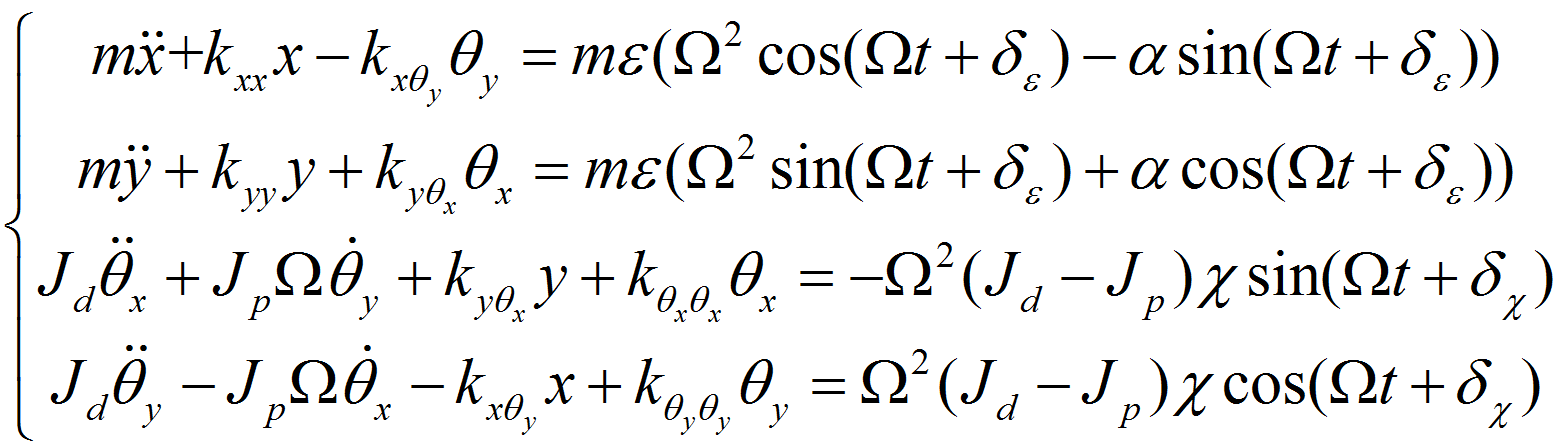
\includegraphics[scale=0.25]{./figures/Images/Math_1}
			\label{math:1}
			\centering
		\end{equation}
		\begin{figure}[h]
			
			\begin{subfigure}[b]{.5\textwidth}
 				\centering
 				 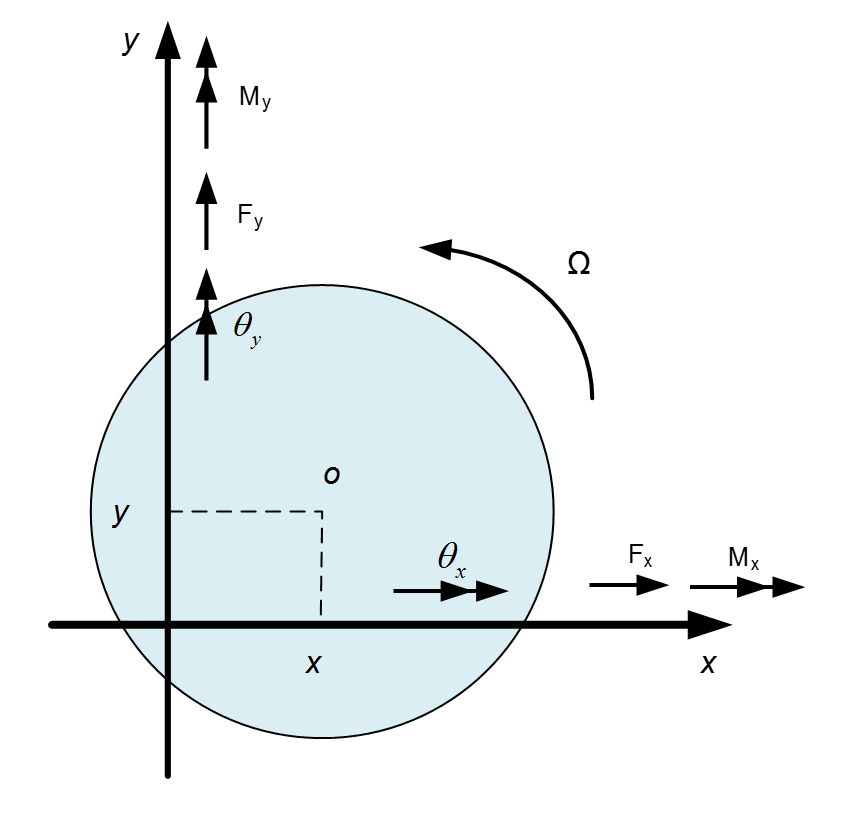
\includegraphics[width=.75\linewidth]{./figures/Images/Figure_1a}
 				 \caption{Displacements, rotations, forces and moments}
 				 \label{fig:Figure_1a}
 				 \centering
			\end{subfigure}%
			\begin{subfigure}[b]{.5\textwidth}
  				\centering
  				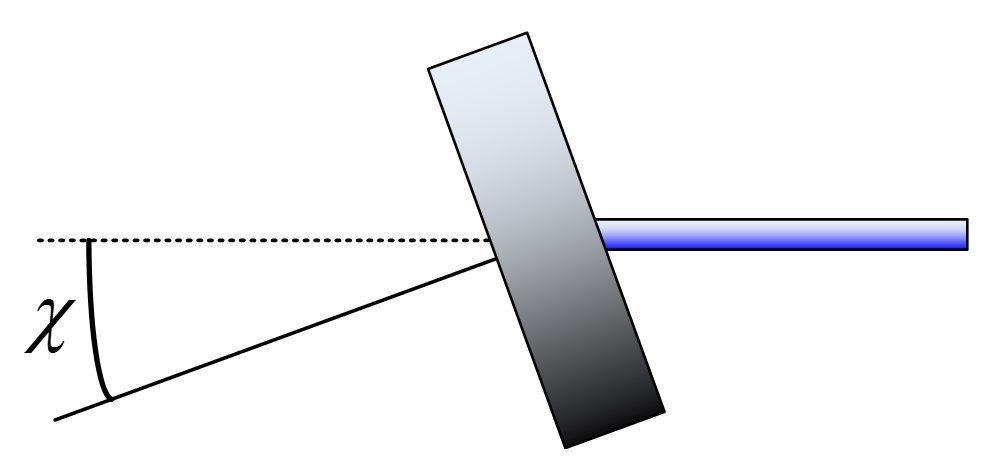
\includegraphics[width=.75\linewidth]{./figures/Images/Figure_1b}
  				\caption{Depiction of skew angle $\chi$}
  				\label{fig:Figure_1b}
  				\centering
			\end{subfigure}
			\caption{Experimental apparatus mathematical representation}
			\label{fig:Figure_1}
			
		\end{figure}
		\begin{figure}[h]
			\centering
			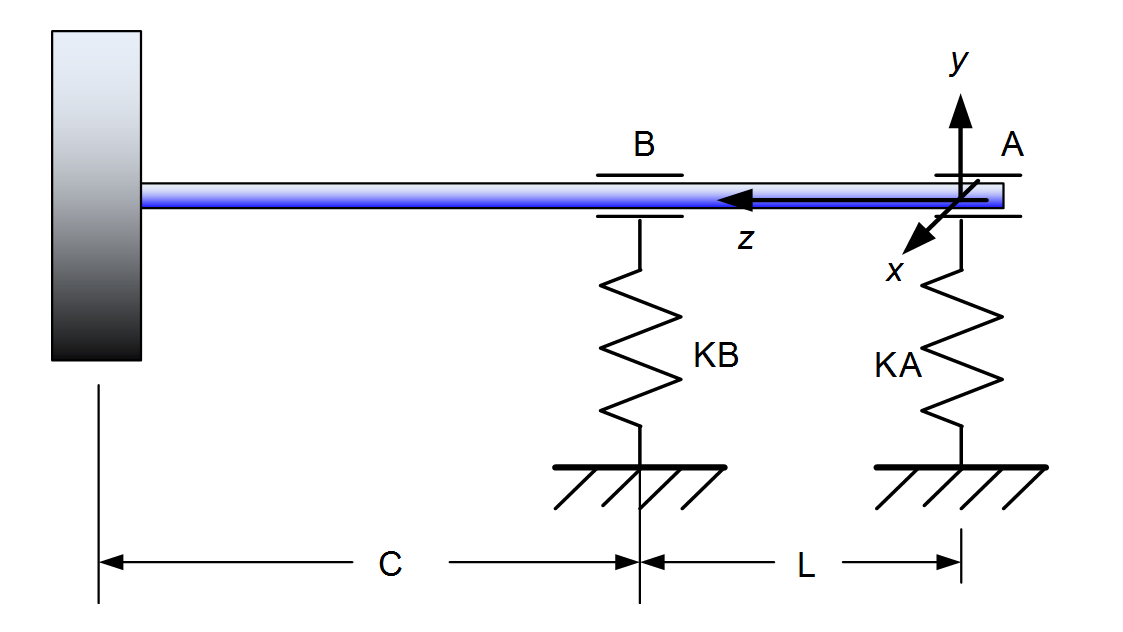
\includegraphics[scale=.25]{./figures/Images/Figure_2}
			\caption{Diagram showing important parameters}
			\label{fig:Figure_2}
			\centering
		\end{figure}
		The total stiffness constants of the system are determined from geometry and properties of the rotor bearings, and divided into two main contributions from the bending of the shaft and the suspension of the bearings. These two contributions are considered independent to solve for each contribution and then are combined in series to determine the total stiffness.\par
		Case (A) Flexible shaft with rigid bearings. Flexible Influence coefficients method in the general form of \ref{math:2} is used to derive flexibility matrix  which can be applied in both $xz$ and $yz$ plane, respectively. Since the shaft is considered to be isotropic, the matrix is identical for the xz and the $yz$ plane (\cite{Ishida},\cite{Dimarogonas}).\par
		\begin{equation}
			\centering
			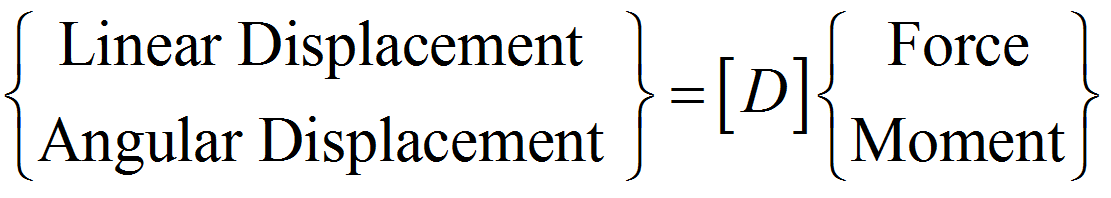
\includegraphics[scale=.25]{./figures/Images/Math_2}
			\label{math:2}
			\centering
		\end{equation}
		\begin{equation}
			\centering
			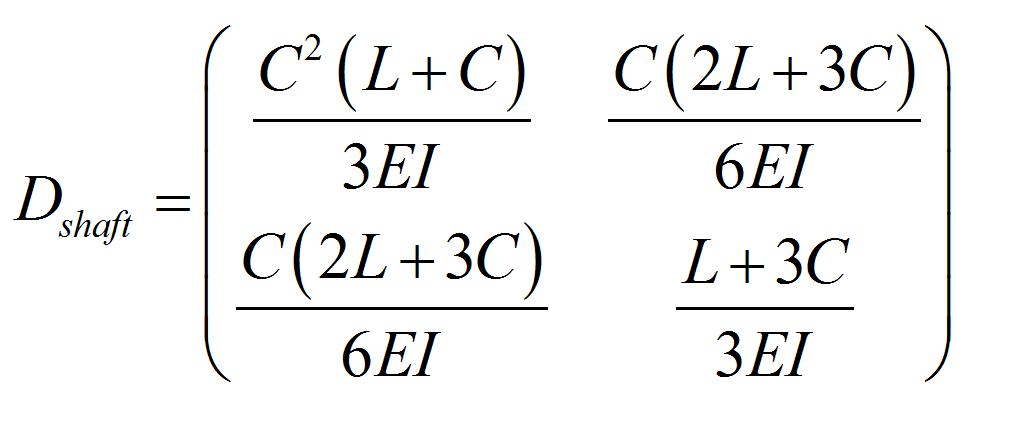
\includegraphics[scale=.25]{./figures/Images/Math_3}
			\label{math:3}
			\centering
		\end{equation}
		Case (B) Rigid shaft with flexible bearing. The stiffness matrix is derived in the general form of \ref{math:4} using stiffness influence coefficients method.\par
		\begin{equation}
			\centering
			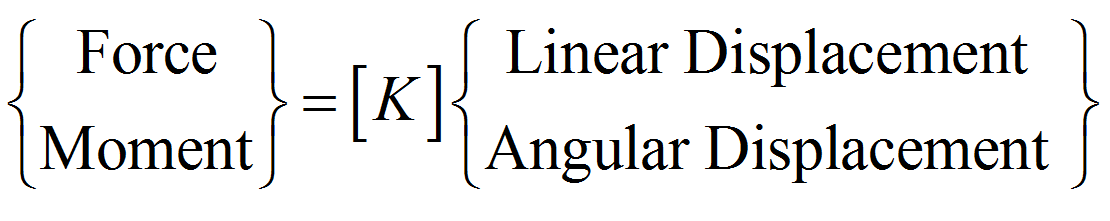
\includegraphics[scale=.25]{./figures/Images/Math_4}
			\label{math:4}
			\centering
		\end{equation}
		\begin{equation}
			\centering
			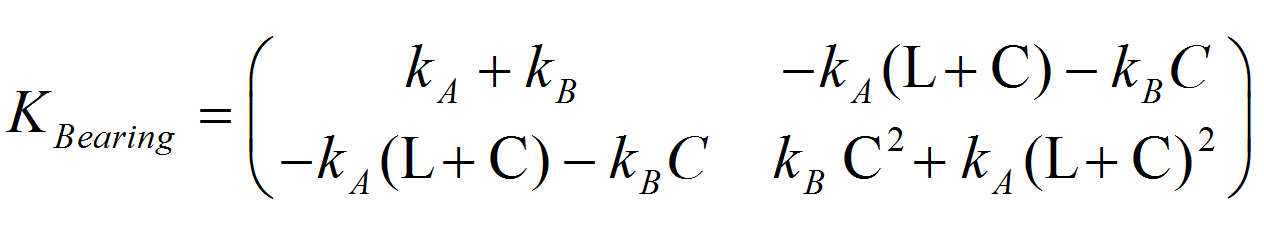
\includegraphics[scale=.25]{./figures/Images/Math_5}
			\label{math:5}
			\centering
		\end{equation}
		In order to combine the bearing stiffness with the shaft stiffness, both are added as flexibility matrices.\par
		\begin{equation}
			\centering
			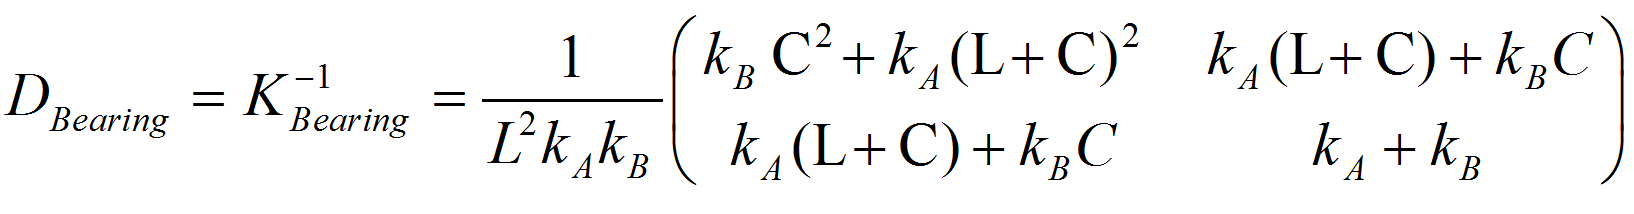
\includegraphics[scale=.25]{./figures/Images/Math_6}
			\label{math:6}
			\centering
		\end{equation}
		Apply to $xz$ and $yz$ plane, respectively to account for anisotropy of bearing stiffness for different planes.\par
		\begin{equation}
			\centering
			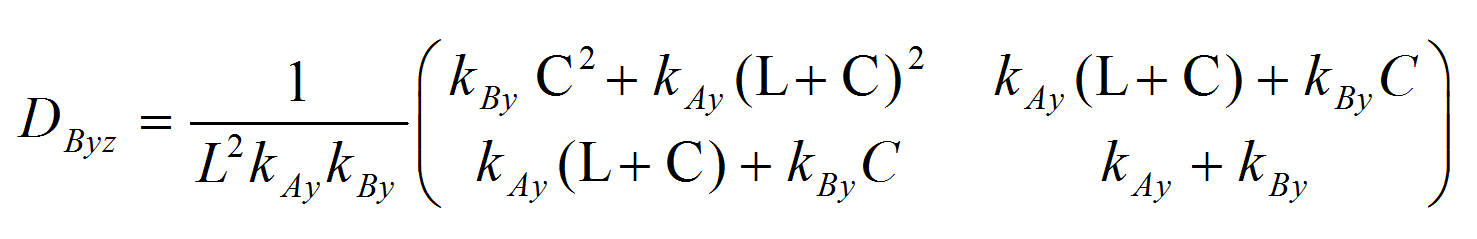
\includegraphics[scale=.25]{./figures/Images/Math_7}
			\label{math:7}
			\centering
		\end{equation}
		\begin{equation}
			\centering
			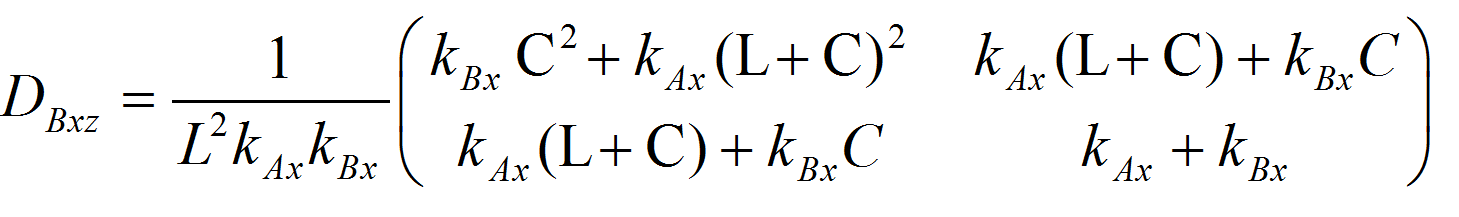
\includegraphics[scale=.25]{./figures/Images/Math_8}
			\label{math:8}
			\centering
		\end{equation}
		Total flexibility matrices in $xz$ and $yz$ plane are:\par
		\begin{equation}
			\centering
			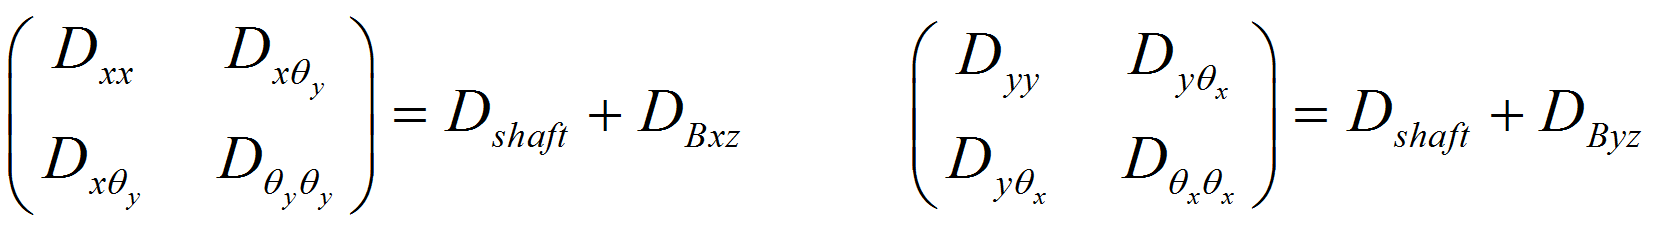
\includegraphics[scale=.25]{./figures/Images/Math_9}
			\label{math:9}
			\centering
		\end{equation}
		Total stiffness matrices are shown in \ref{math:10}, which are applied in equations of motion \ref{math:1}.\par
		\begin{equation}
			\centering
			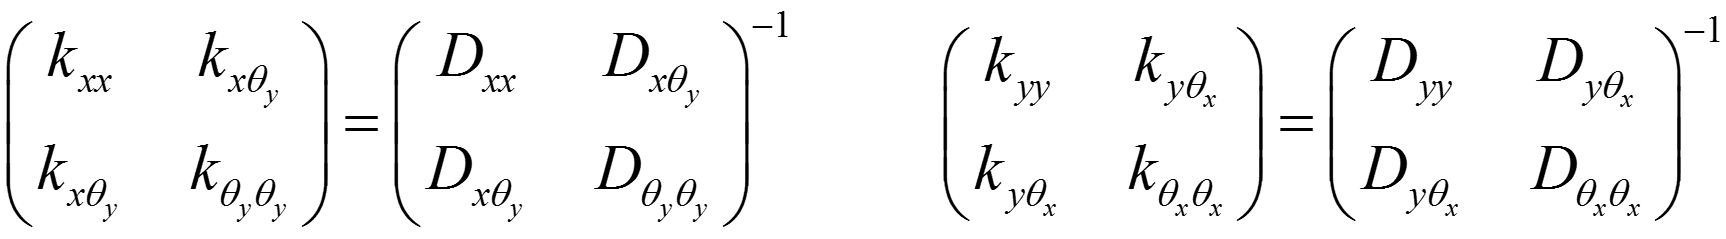
\includegraphics[scale=.25]{./figures/Images/Math_10}
			\label{math:10}
			\centering
		\end{equation}
			
	\section{Experimental apparatus}
		Our experimental apparatus consists of the GE (Formally Bently Nevada) RK4 rotor kit, the ADRE 408 Dspi Data asset condition monitoring equipment, and a laptop with the ADRE sxp software (Figure \ref{fig:Figure_3}). Four eddy current displacement transducers are used to measure the vibration of the shaft. The ADRE 408, when coupled with ADRE sxp, is capable of providing real-time signal processing from the rotor system in meaningful figures.\par
		\begin{figure}[H]
			\begin{subfigure}[b]{.5\textwidth}
				\centering
				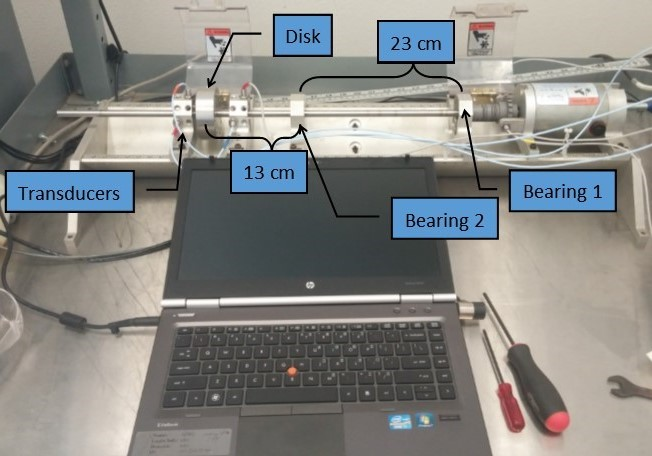
\includegraphics[width=.95\linewidth]{./figures/Images/Figure_3.jpg}
				\caption{Schematic of rotor geometry}
				\label{fig:Figure_3a}
				\centering
			\end{subfigure} %
			\begin{subfigure}[b]{.5\textwidth}
				\centering
				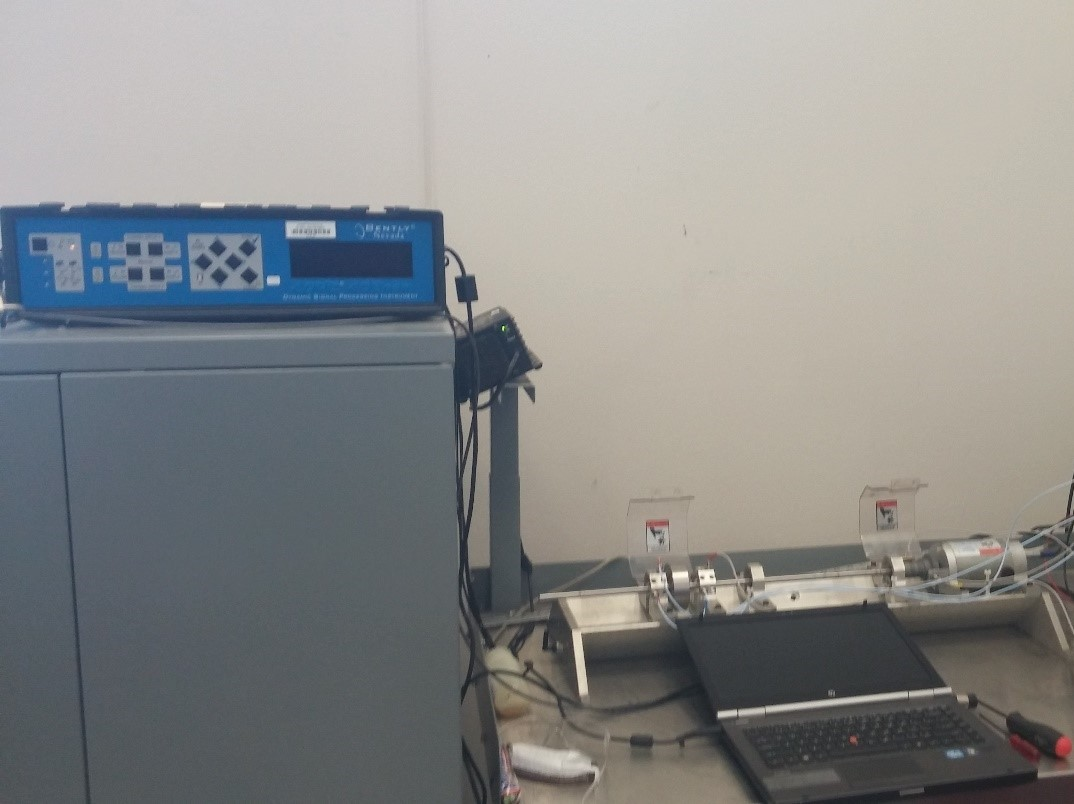
\includegraphics[width=.95\linewidth]{./figures/Images/Figure_3b.jpg}
				\caption{Overview of apparatus}
				\label{fig:Figure_3b}
				\centering
			\end{subfigure}
			\caption{Experimental apparatus}
			\label{fig:Figure_3}
		\end{figure}
		\begin{table}[H]
			\centering
			\caption{Rotor parameters}
			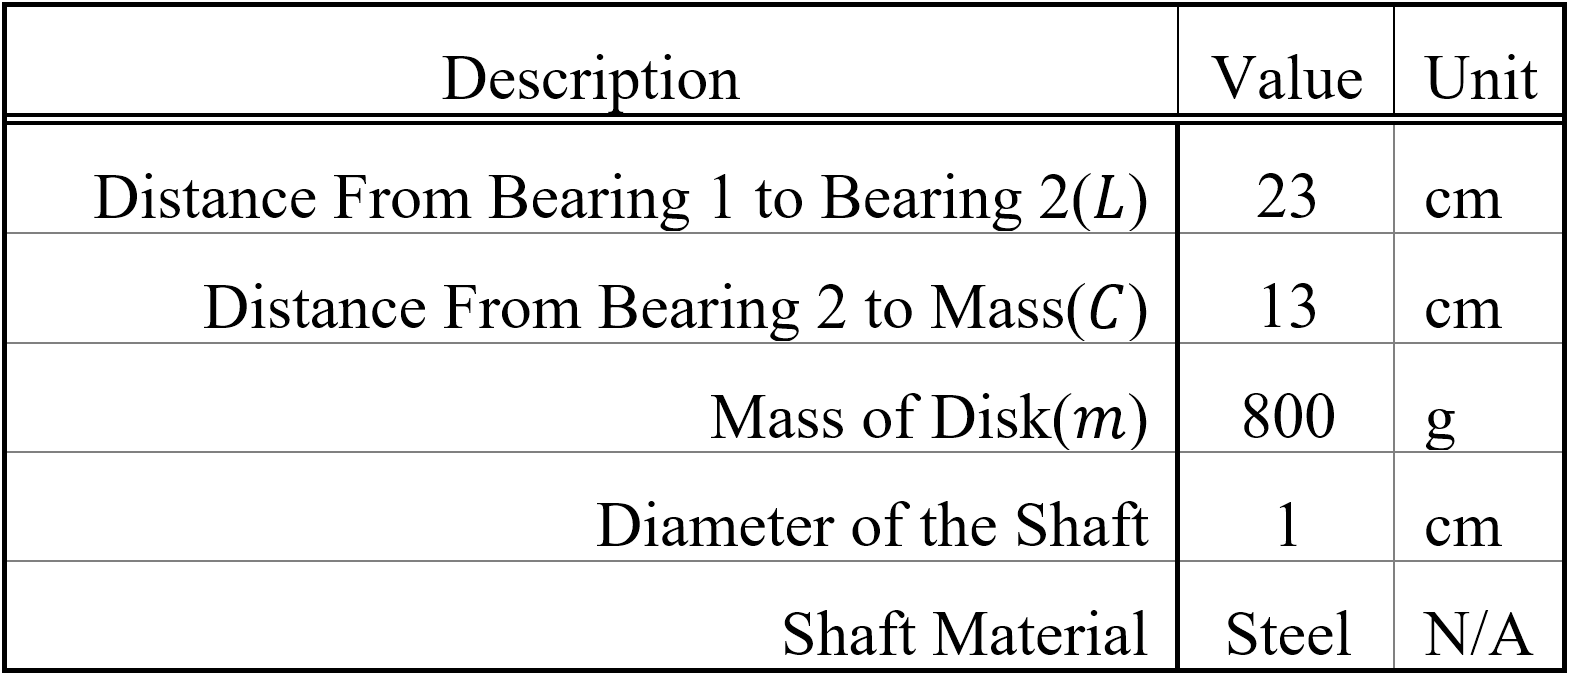
\includegraphics[scale=.25]{./figures/Images/Table_1}
			\label{tab:Table_1}
			\centering
		\end{table}
	\section{Identify the bearing stiffness parameters from experimental data}
		With the experimental data we were able to identify the natural frequency in the horizontal and vertical directions from the Bode plot of each horizontal and vertical transducer. From the theoretical equations of motion, the eigenvalue problem can be used to solve for the natural frequencies of the system. Since the system includes gyroscopic moments that depend on the rotational speed of the rotor, the natural frequency is a function of the speed of the rotor. The Campbell Diagram is a plot of the natural frequency as it changes with the increasing speed of the rotor. This diagram can be used to tune the bearing stiffness. The parameters that affect the natural frequency that are not evident from the description of the system is the stiffness of the bearings in each $xz$ and $yz$ plane. To solve for the stiffness values, a Campbell Diagram is created for each value of stiffness until the point at which the natural frequency line intersects the rotor speed line is the same value as the experimental natural frequency. An example of a Campbell diagram can be seen in Figure \ref{fig:Figure_4}. The Campbell diagram gives a good depiction of how the natural frequency changes with speed and how negative natural frequencies decrease in frequency, while the positive natural frequency increases. The stiffness of the bearings was determined to be about 91000 N/m in the xz plane and about 120000 N/m in the $yz$ plane.\par 
		\begin{figure}[H]
			\centering
			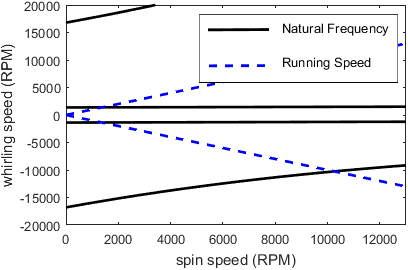
\includegraphics[scale=.75]{./figures/Images/Figure_4}
			\caption{Example Campbell diagram}
			\label{fig:Figure_4}
		\end{figure}
		To further understand the effect that stiffness anisotropy has on the system, Figure \ref{fig:Figure_5} and \ref{fig:Figure_6}  display a cascade of amplitude plots with changing stiffness anisotropy between the horizontal and vertical planes. Viewing the theoretical data in this way allows for comparison of the two natural frequencies to experimental values just as the Campbell Diagram does. In addition, the cascaded plots depict how the shape of the amplitude plots change with varying anisotropy. Figure \ref{fig:Figure_5}  uses the amplitude of positive and negative frequencies to display the effect of anisotropy. The interaction between the first and second natural frequencies can be seen as the two get closer to one another. Negative whirling is dominant only between the two natural frequencies. When the two natural frequencies coincide, there is a highly circular positive whirl orbit. Experimental amplitude plots are used in conjunction with Figure \ref{fig:Figure_5}  \& \ref{fig:Figure_6}  to choose the correct anisotropy at which the characteristic shape matches.\par 
		The skew angle, $\chi$, and the eccentricity, $\varepsilon$, are determined next by independent methods. Eccentricity can be determined by simulating the theoretical model under varying eccentricities until the magnitude of the vibration is equivalent to that of the experimental results. The value was determined to be $9\e{-4}  m$. The skew angle can be quantified using a similar technique. But the skew angle is closely related to the amplitude of vibration in the two orthogonal directions, $x$ and $y$, as well as the disk tilting angles, $\theta_x$ and $\theta_y$. In order to measure the tilting angles in the experiment, there were two sets of orthogonal transducers. One before the disk on the shaft and the other after the disk. This displacement between the two sets of transducers allows for an approximation of the angles of tilt. Assuming no bending of the shaft, the angle is deduced from a pivot about Bearing B, with the angle being equal to the inverse tangent of the ratio of difference in displacement between the transducers, and the distance between the transducers. Then the simulation is run with varying values of $\chi$ to match the amplitude of angles and displacements to the experiment. The value was determined to be 0.09 radians.\par 
		\begin{figure}[H]
			\centering
			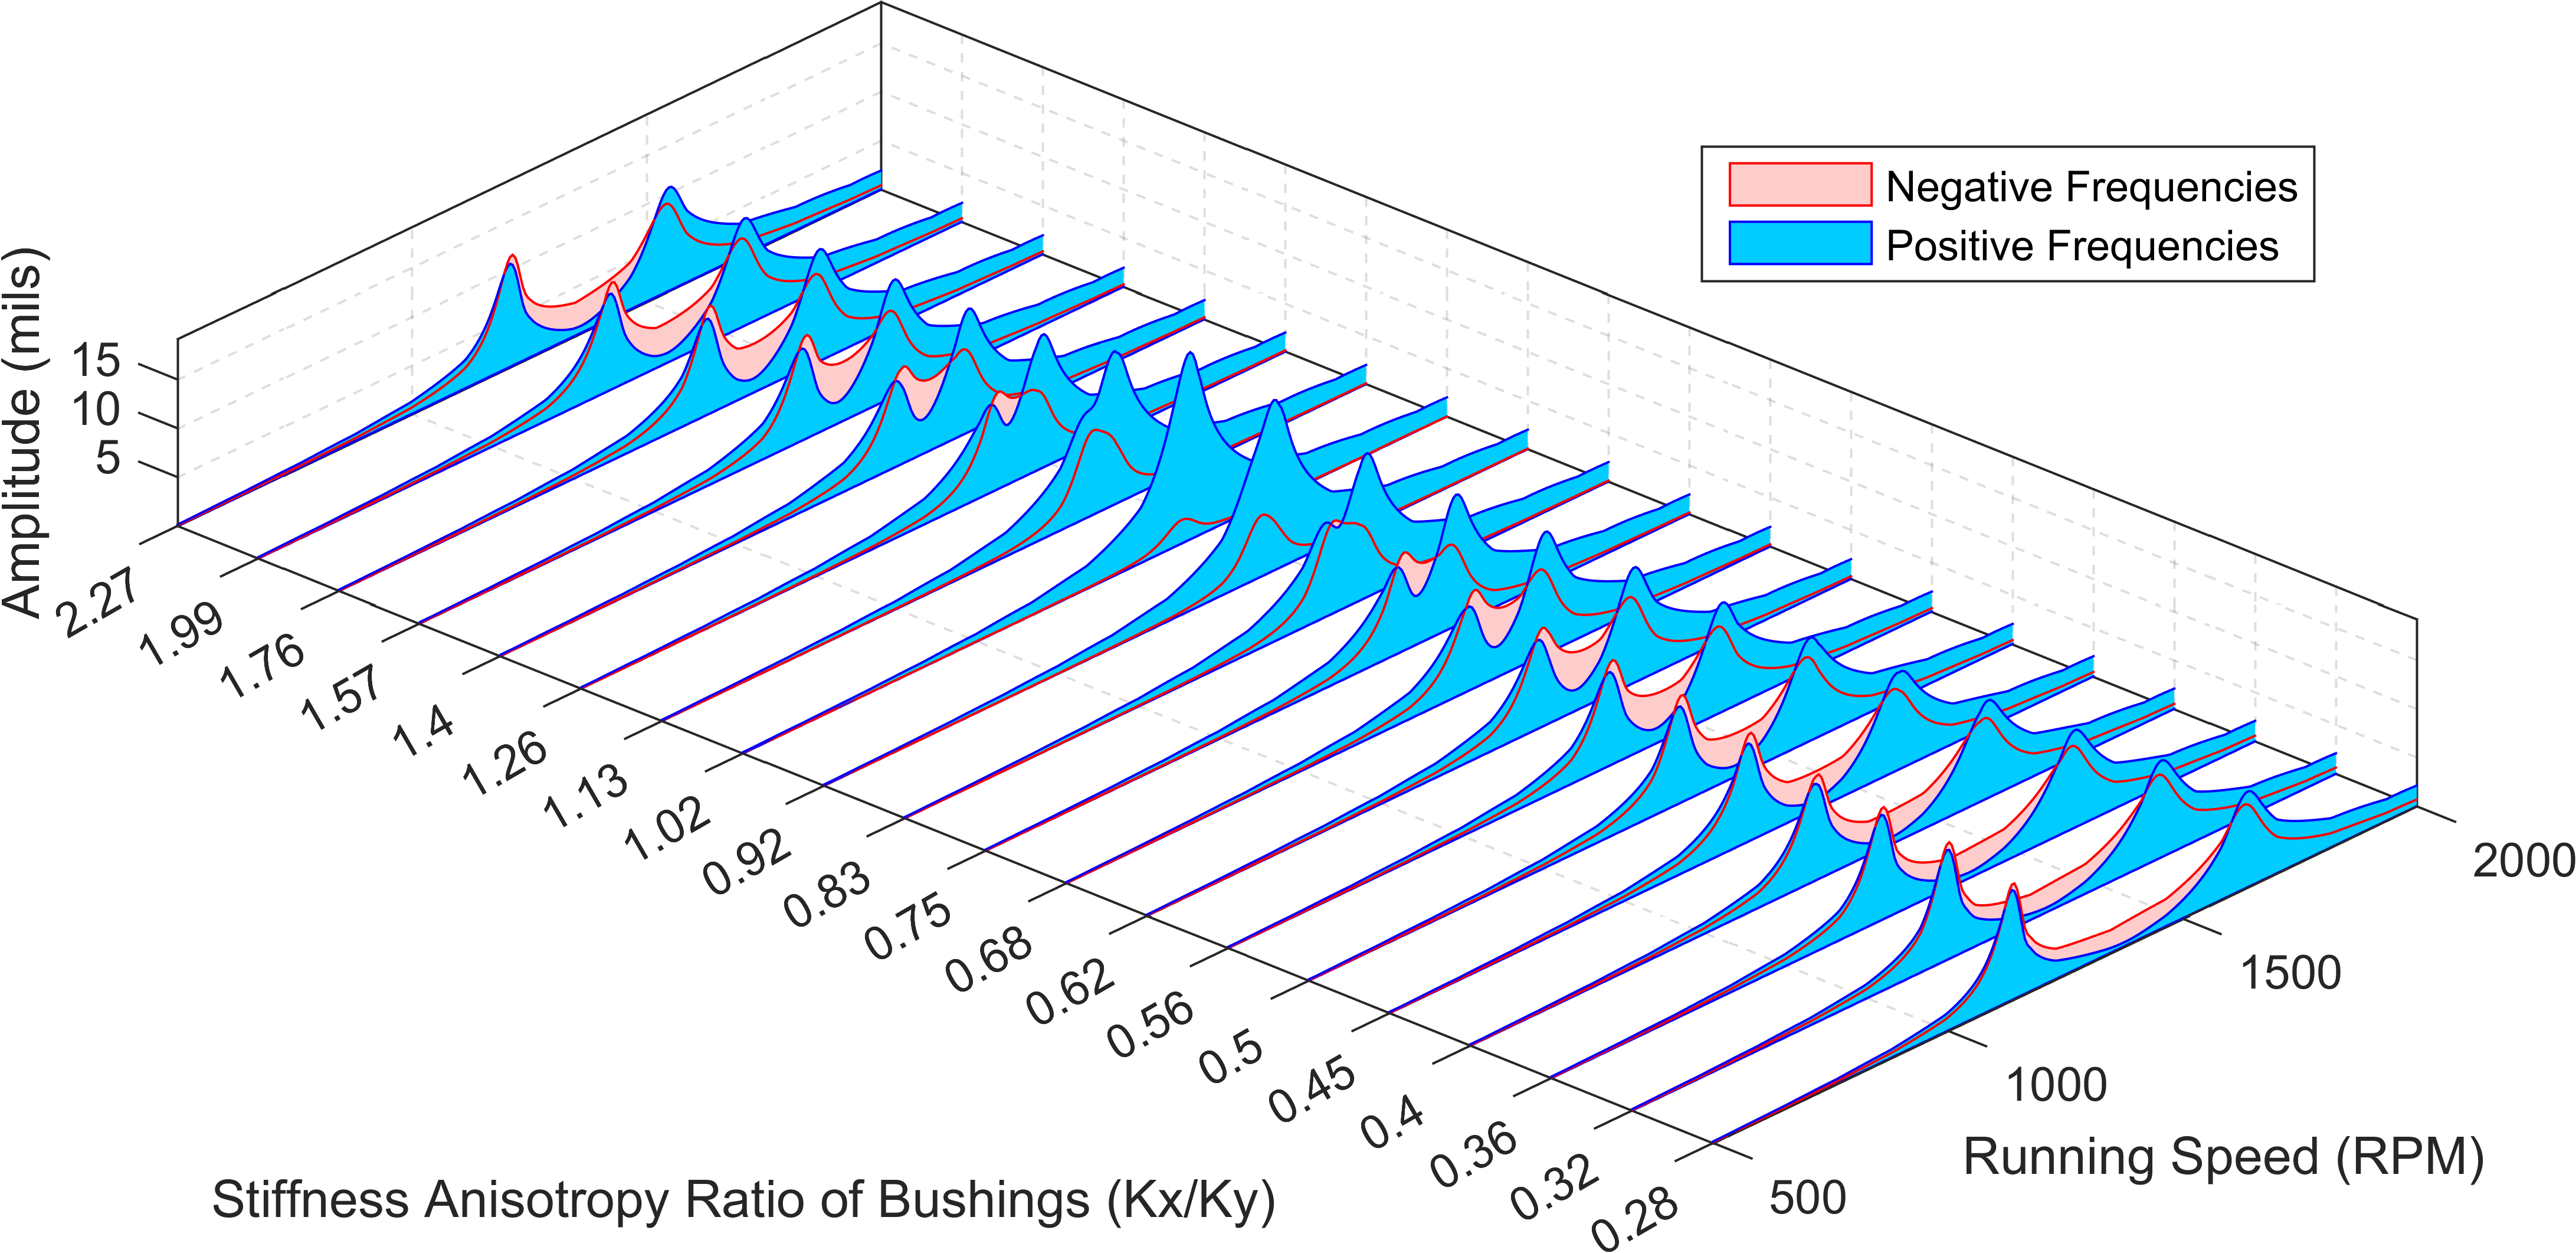
\includegraphics[width=.75\linewidth]{./figures/Images/Figure_5}
			\caption{3D cascading plot demonstrating the impact of stiffness anisotropy on positive/negative frequencies}
			\label{fig:Figure_5}
		\end{figure}
		\begin{figure}[H]
			\centering
			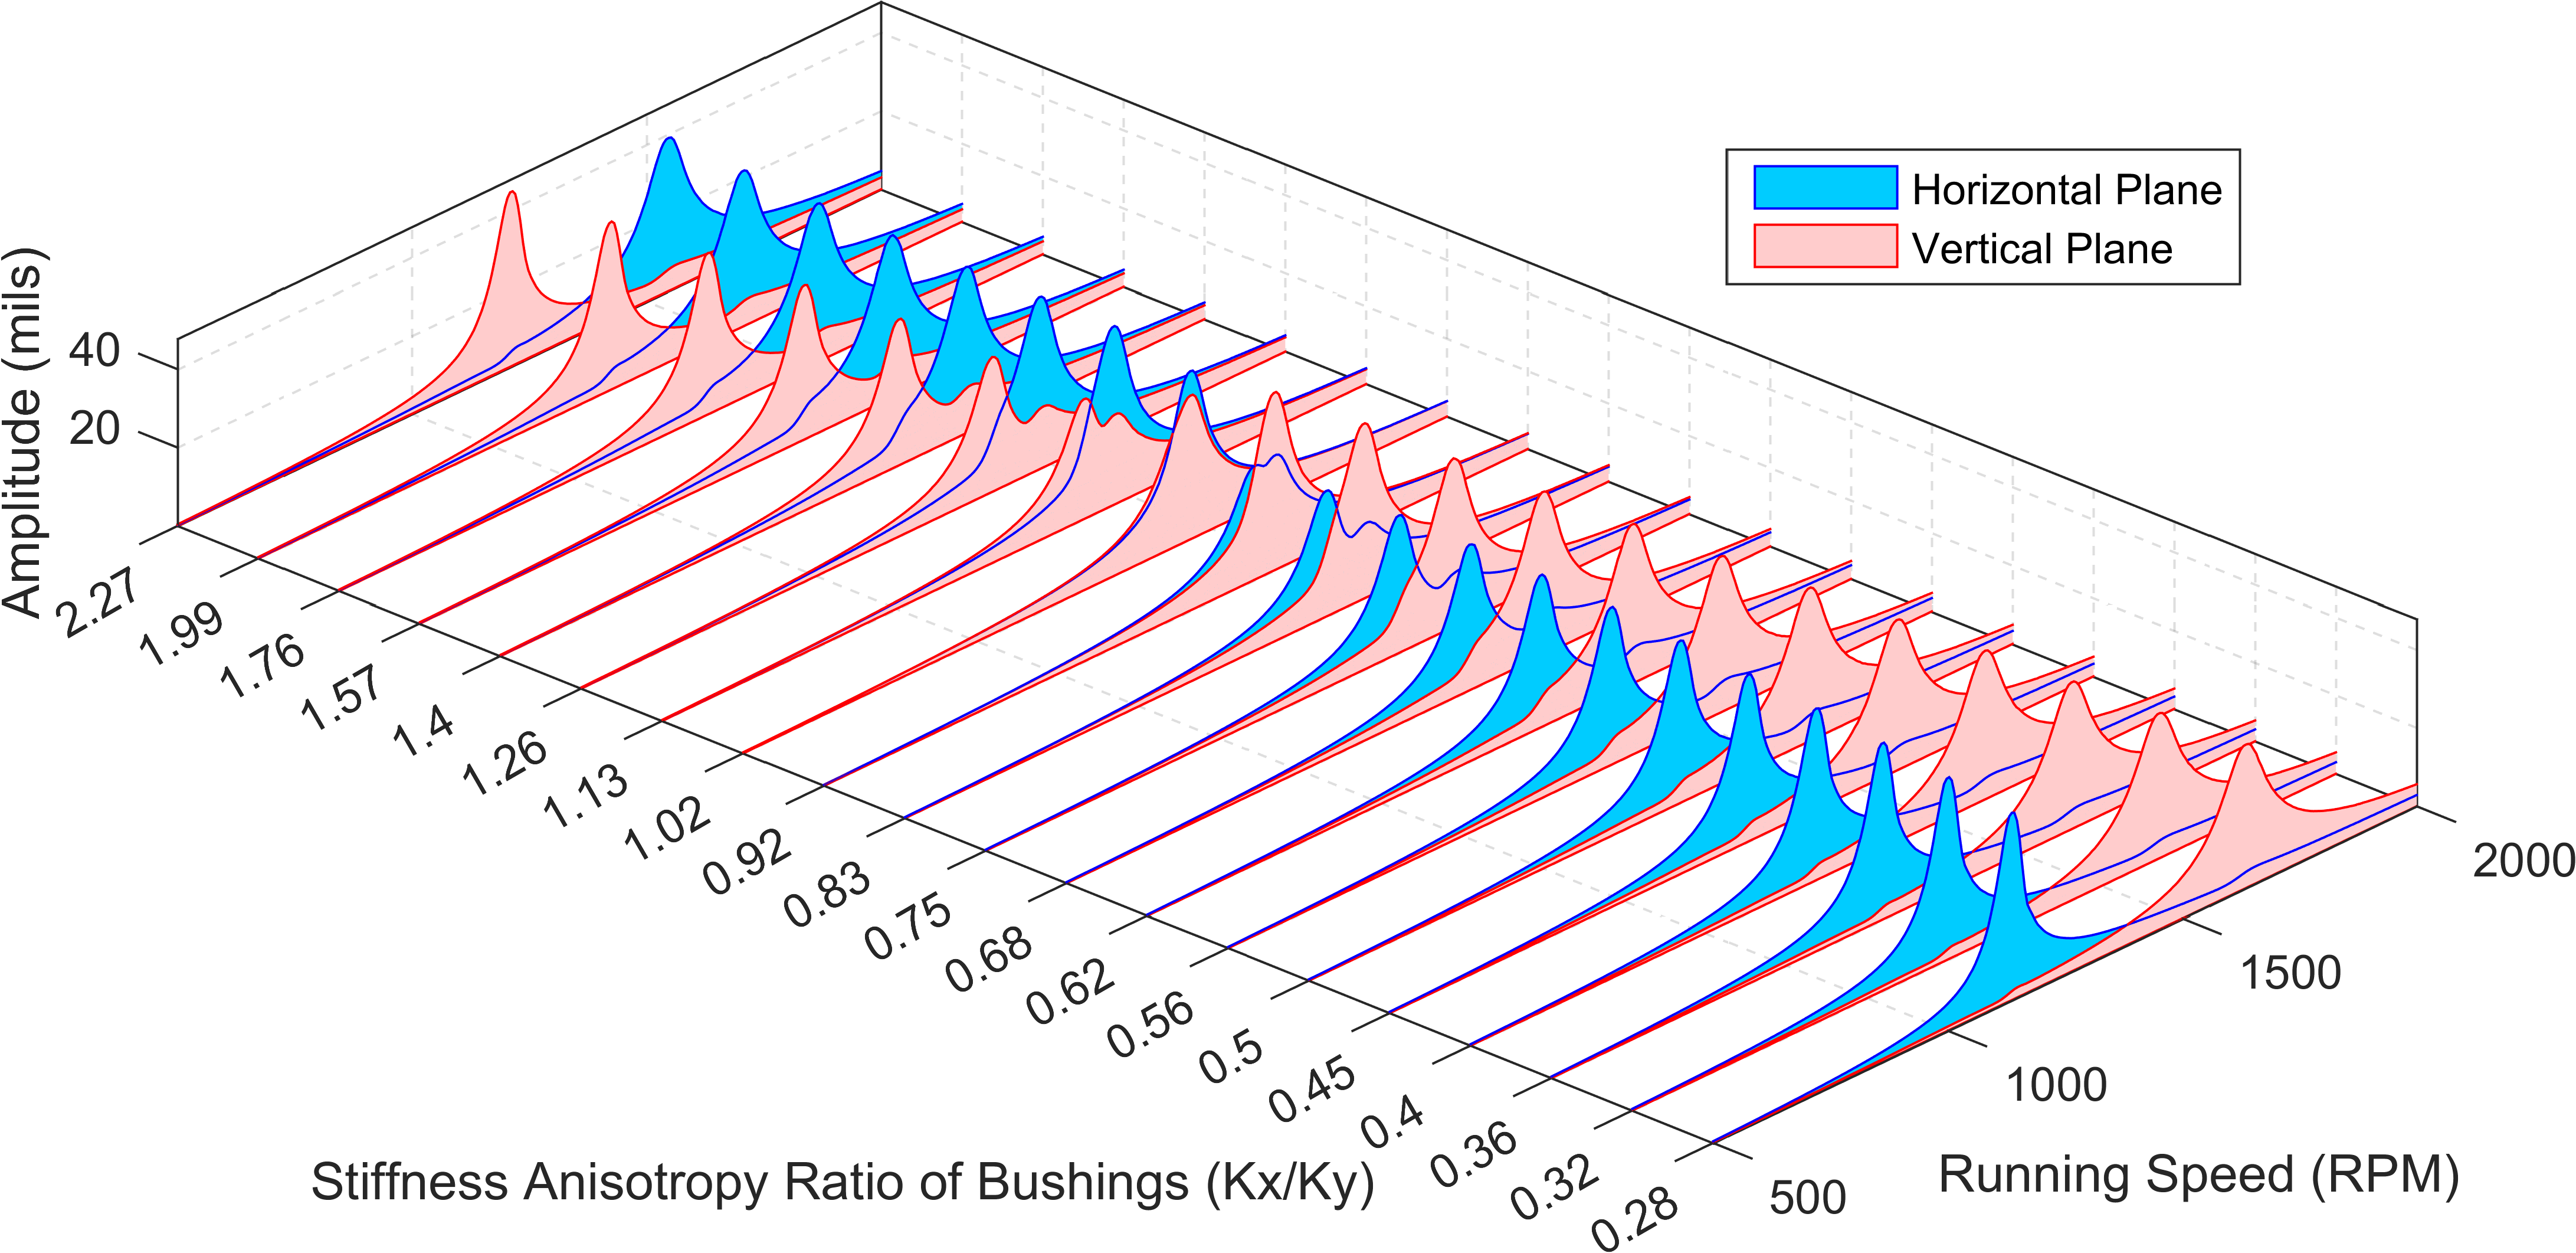
\includegraphics[width=.75\linewidth]{./figures/Images/Figure_6}
			\caption{3D cascading plot demonstrating the impact of stiffness anisotropy on horizontal/vertical frequencies}
			\label{fig:Figure_6}
		\end{figure}

	\section{Produce full spectrum plots from orthogonal transducers }
		The purpose of this work was to produce figures that represent vibration amplitude data from theoretical models in a way that is comparable to figures produced by the ADRE Sxp software. This allows the analysis of theoretical models with confidence in the representation of the data with figures such as the Bode plot, the Cascade plot, and full spectrum plots. The major achievement in producing the figures was obtaining phase lag angles between two signals. Another achievement was producing spectrum plots with both positive and negative frequencies (Full Spectrum plots).\par 
		Full spectrum plots are more complete in displaying the information contained in a Fourier Transform. In the frequency domain, negative frequencies pertain to vibration of the rotor that is precessing in the opposite rotational direction than that of the rotor rotational direction. The full spectrum plot is produced by first coupling the orthogonal transducer signals into a complex signal and then performing a Fourier transform. The transform on the complex data results in frequency information both negative and positive.\par 
		Negative frequencies tell a lot about the system, especially when they are greater than their positive counterpart. When the negative frequency vibration is greater in amplitude, the precession is said to be in the “reverse” direction. This can be vital information in diagnosing a problem in a real rotor system. In the case explored here it can be a sign of both, strong gyroscopic moments, as well as anisotropy of the stiffness from the shaft or the bearings. Another example is the rub in a fluid film bearing which manifests itself as a negative precession at twice the running speed of the rotor. This problem would be more difficult to diagnose without the knowledge of negative frequencies.\par 
		In order to verify that the MATLAB code of our method would produce accurate frequency data, the Fast Fourier Transform, or FFT, of a steady state signal was compared to the FFT produced by the ADRE 408 with ADRE Sxp software. Both the amplitude and frequency of positive and negative frequency components was verified by comparison as demonstrated by the comparison of Figure \ref{fig:Figure_7}  and \ref{fig:Figure_8} .\par 
		\begin{figure}[H]
			\centering
			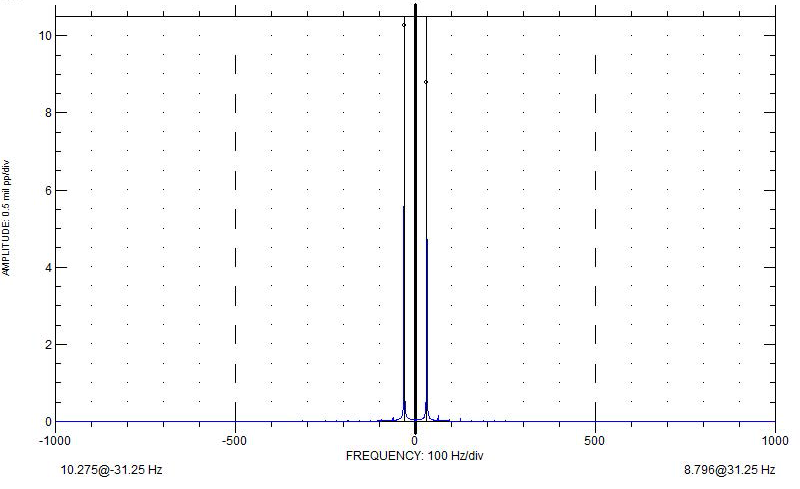
\includegraphics[width=.6\linewidth]{./figures/Images/Figure_7}
			\caption{Full Spectrum plot produced with the ADRE sxp software}
			\label{fig:Figure_7}
		\end{figure}
		\begin{figure}[H]	
			\centering
			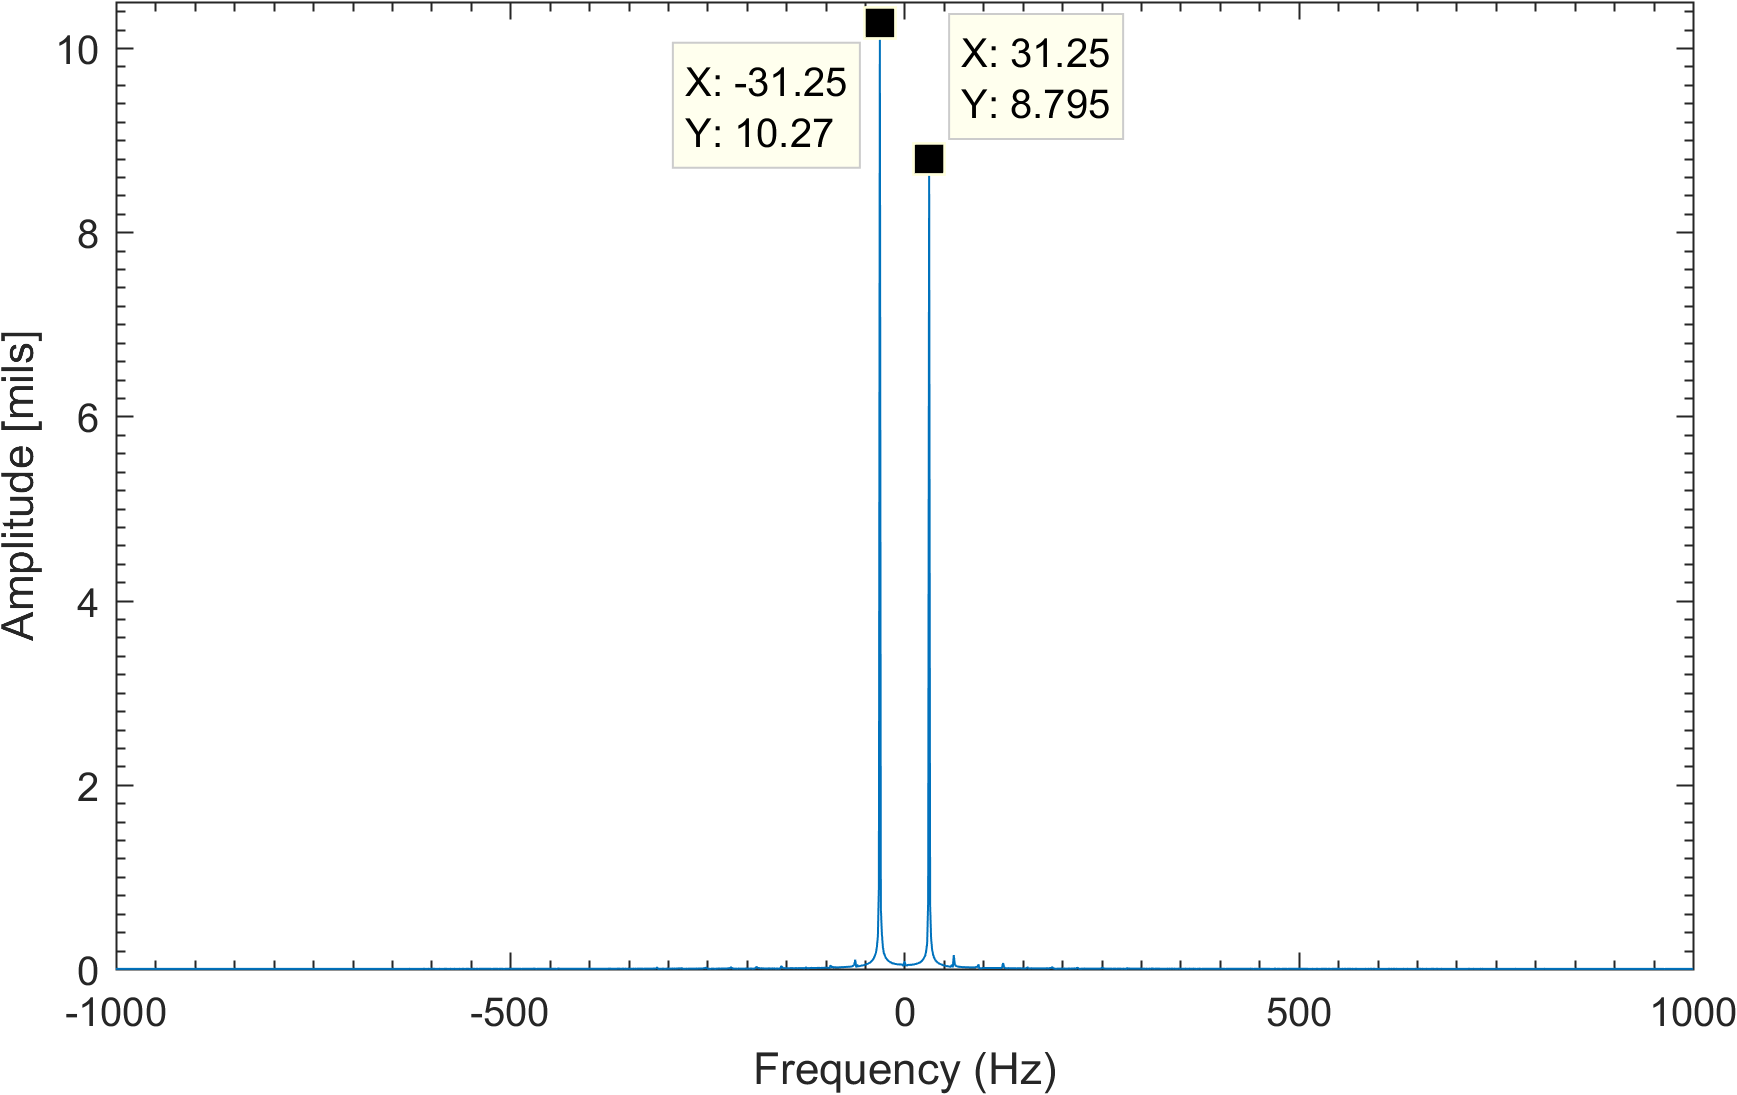
\includegraphics[width=.6\linewidth]{./figures/Images/Figure_8}
			\caption{Full Spectrum plot produced with using our method}
			\label{fig:Figure_8}
		\end{figure}
	\section{Produce Bode plots from orthogonal transducers }
		The process for producing phase lag angles begins with segmenting the data into windows of a fixed number of samples. This is because most rotordynamic data comes in the form of a “start-up” or a “run-down”. In both of these scenarios, the rotational speed of the rotor is continuously changing, as demonstrated by Figure \ref{fig:Figure_9a}. This change deters capturing both time and frequency information. Segmenting the data provides small windows on which analysis can be performed as if the signal was a constant frequency within the window, as demonstrated in Figure \ref{fig:Figure_9b}. For a segment of data in which the frequency is not changing, a Fourier Transform can be applied to obtain the frequency spectrum of the signal. In this frequency domain provided by the Fourier Transform, the phase angle of each frequency can be obtained as well as the amplitude of vibration of each frequency. In order to calculate the phase lag from one signal to another, this phase angle is compared for the same frequency of each signal in the same window in time. This process is done for each window through the entire length of data producing a phase angle for each window.\par 
		The Bode plot is ubiquitous in rotating machinery diagnostics and can be used to characterize a system fairly thoroughly. Phase angle is a vital part of the bode plot and can shed light on many phenomenon One of the main goals in this paper is to demonstrate the ability to produce accurate phase lag information from two signals. As seen in the Bode plot of Figure \ref{fig:Figure_10} , the MATLAB code based on complex FFT strategy produces phase lag information nearly identical to the phase lag information produced with the ADRE system using the same transducer data.\par 
		\begin{figure}[H]
			\begin{subfigure}[b]{.5\linewidth}	
				\centering
				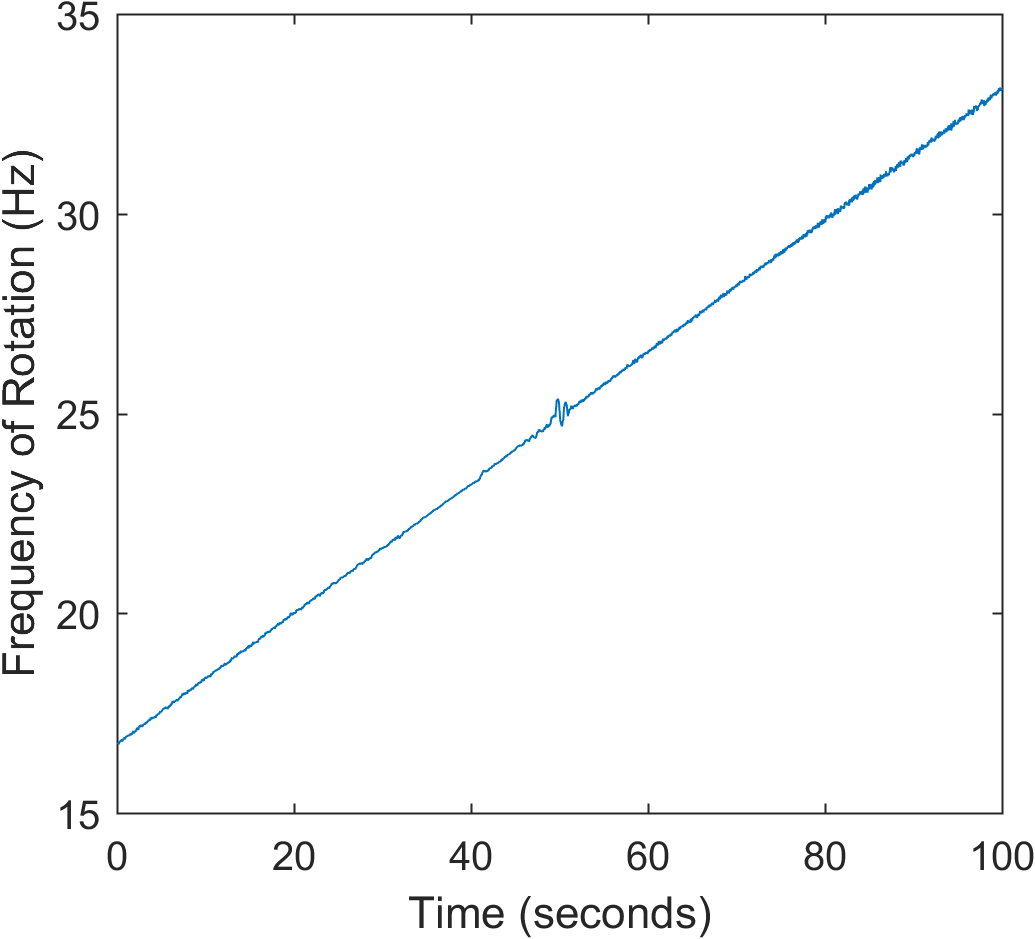
\includegraphics[width=1\textwidth]{./figures/Images/Figure_9a}
				\caption{Rotational speed change over time}
				\label{fig:Figure_9a}
			\end{subfigure}
			\begin{subfigure}[b]{.5\linewidth}
				\centering
				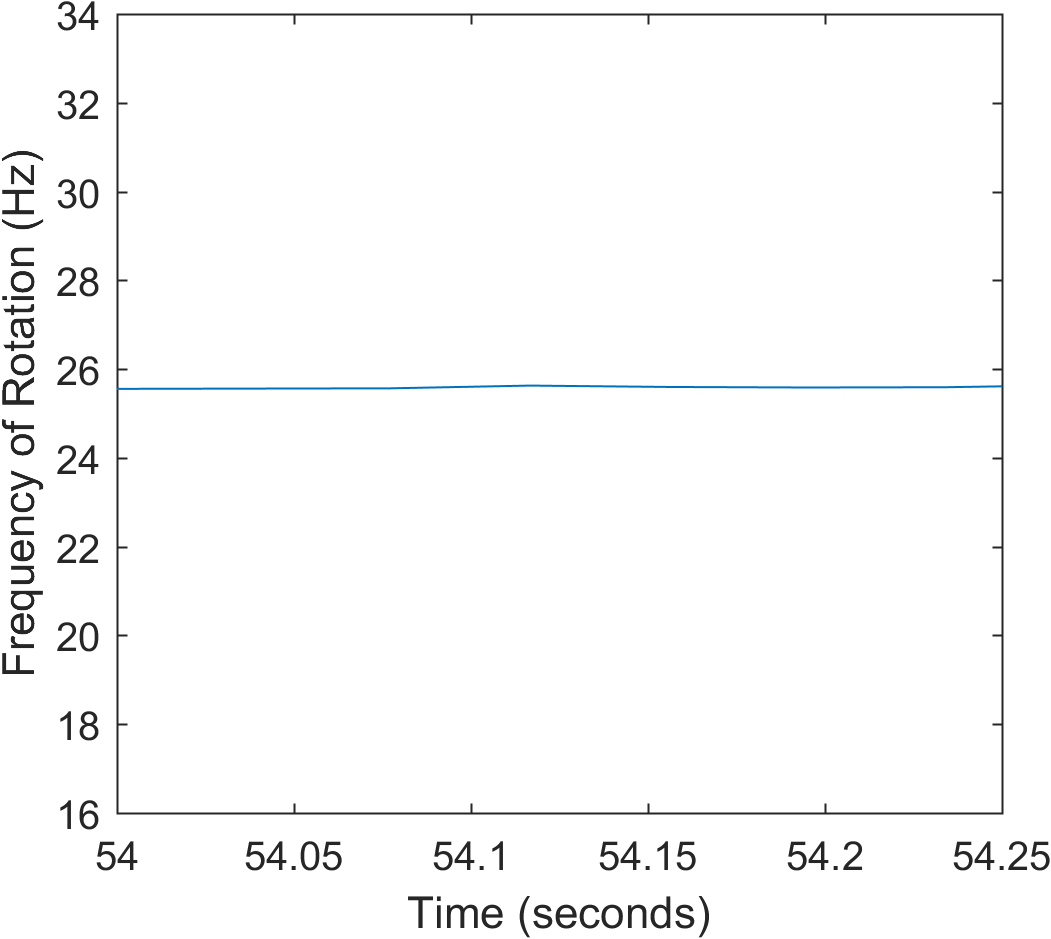
\includegraphics[width=1\textwidth]{./figures/Images/Figure_9b}
				\caption{Rotational speed change over a window in time}
				\label{fig:Figure_9b}
			\end{subfigure}
			\caption{Steady-state approximation demonstration}
			\label{fig:Figure_9}
		\end{figure}
		This ability to produce phase lag information from any transducer data allows accurate comparison of theoretical and experimental data. The MATLAB code that produces these plots also allows the ability of tuning the resolution of the phase and amplitude information, gaining accuracy in either time or frequency. The phase lag calculation accuracy is determined by the number of cycles analyzed in each window, so the larger the window, the better the phase information. But, as the window gets larger, the accuracy of speed is diminished.\par 
		\begin{figure}[H]	
			\centering
			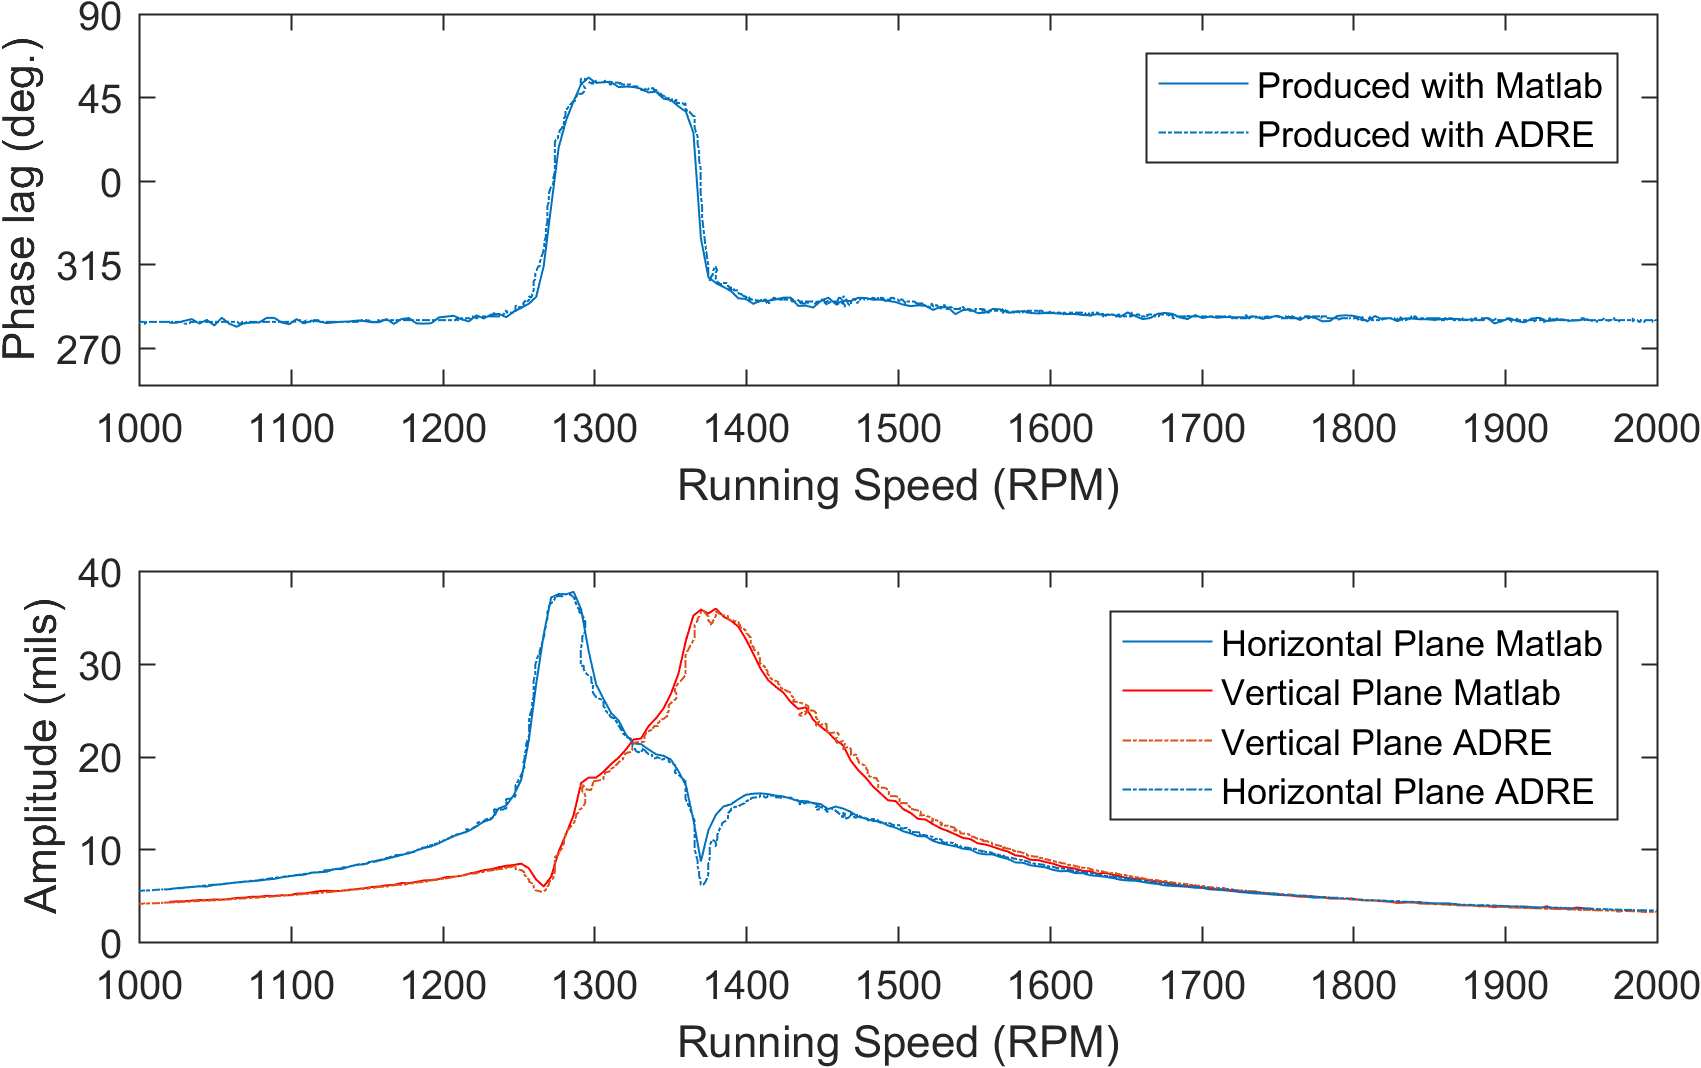
\includegraphics[width=.75\linewidth]{./figures/Images/Figure_10}
			\caption{Bode plot for verification of the phase angle technique}
			\label{fig:Figure_10}
		\end{figure}
	\section{Theoretical and experimental comparison}
		The comparison of experiment and theoretical model developed in this research were performed. The geometric and other parameters of the rotor kit are shown in table 1.\par 
		\begin{figure}[H]	
			\centering
			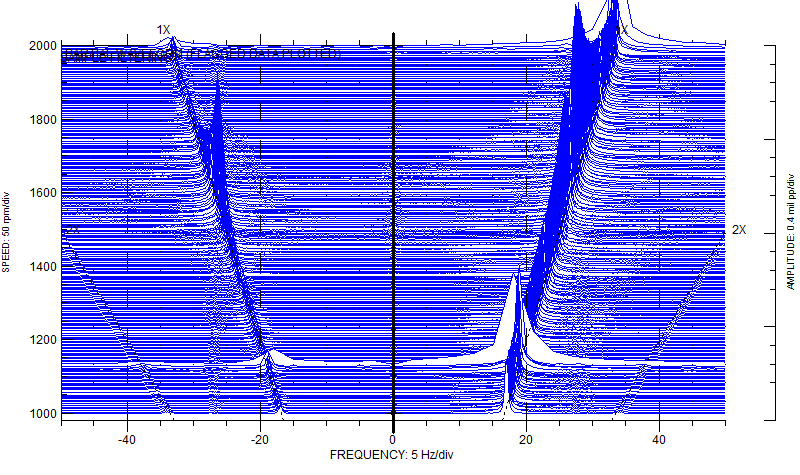
\includegraphics[width=.75\linewidth]{./figures/Images/Figure_11}
			\caption{Experimental Cascade plot directly produced by the ADRE sxp software}
			\label{fig:Figure_11}
		\end{figure}
		\begin{figure}[H]	
			\centering
			\includegraphics[width=.75\linewidth]{./figures/Images/Figure_12}
			\caption{Re-constructed 3D experimental full-spectrum cascade plot using our strategy}
			\label{fig:Figure_12}
		\end{figure}
		\begin{figure}[H]	
			\centering
			\includegraphics[width=.75\linewidth]{./figures/Images/Figure_13}
			\caption{3D theoretical full-spectrum cascade plot using our strategy}
			\label{fig:Figure_13}
		\end{figure}
		The full-spectrum cascade plot is a vital tool for analysis in rotating machinery. The cascade plot depicts how the vibrations change with time. With the addition of the full spectrum in these cascade plots, the negative frequencies provide insight for diagnostics of certain rotor issues, such as misalignment of disk axis with the rotor axis. Just as with the FFT and Bode plots, the cascade plot produced with our MATLAB code using complex FFT strategy is compared with the cascade produced with the ADRE software to validate the method. From figure \ref{fig:Figure_11}, \ref{fig:Figure_12} and \ref{fig:Figure_13}, we can see the results are similar and good enough to validate our full-spectrum strategy through experiment. Furthermore, MATLAB has the ability to display data in three dimensions as shown in the figures (\cite{Southwick},\cite{Southwick 94},\cite{Dimarogonas}). With proper tuning of window size and sampling frequency, the cascade plot can display a host of rotordynamic phenomenon.\par 
		\begin{figure}[H]	
			\centering
			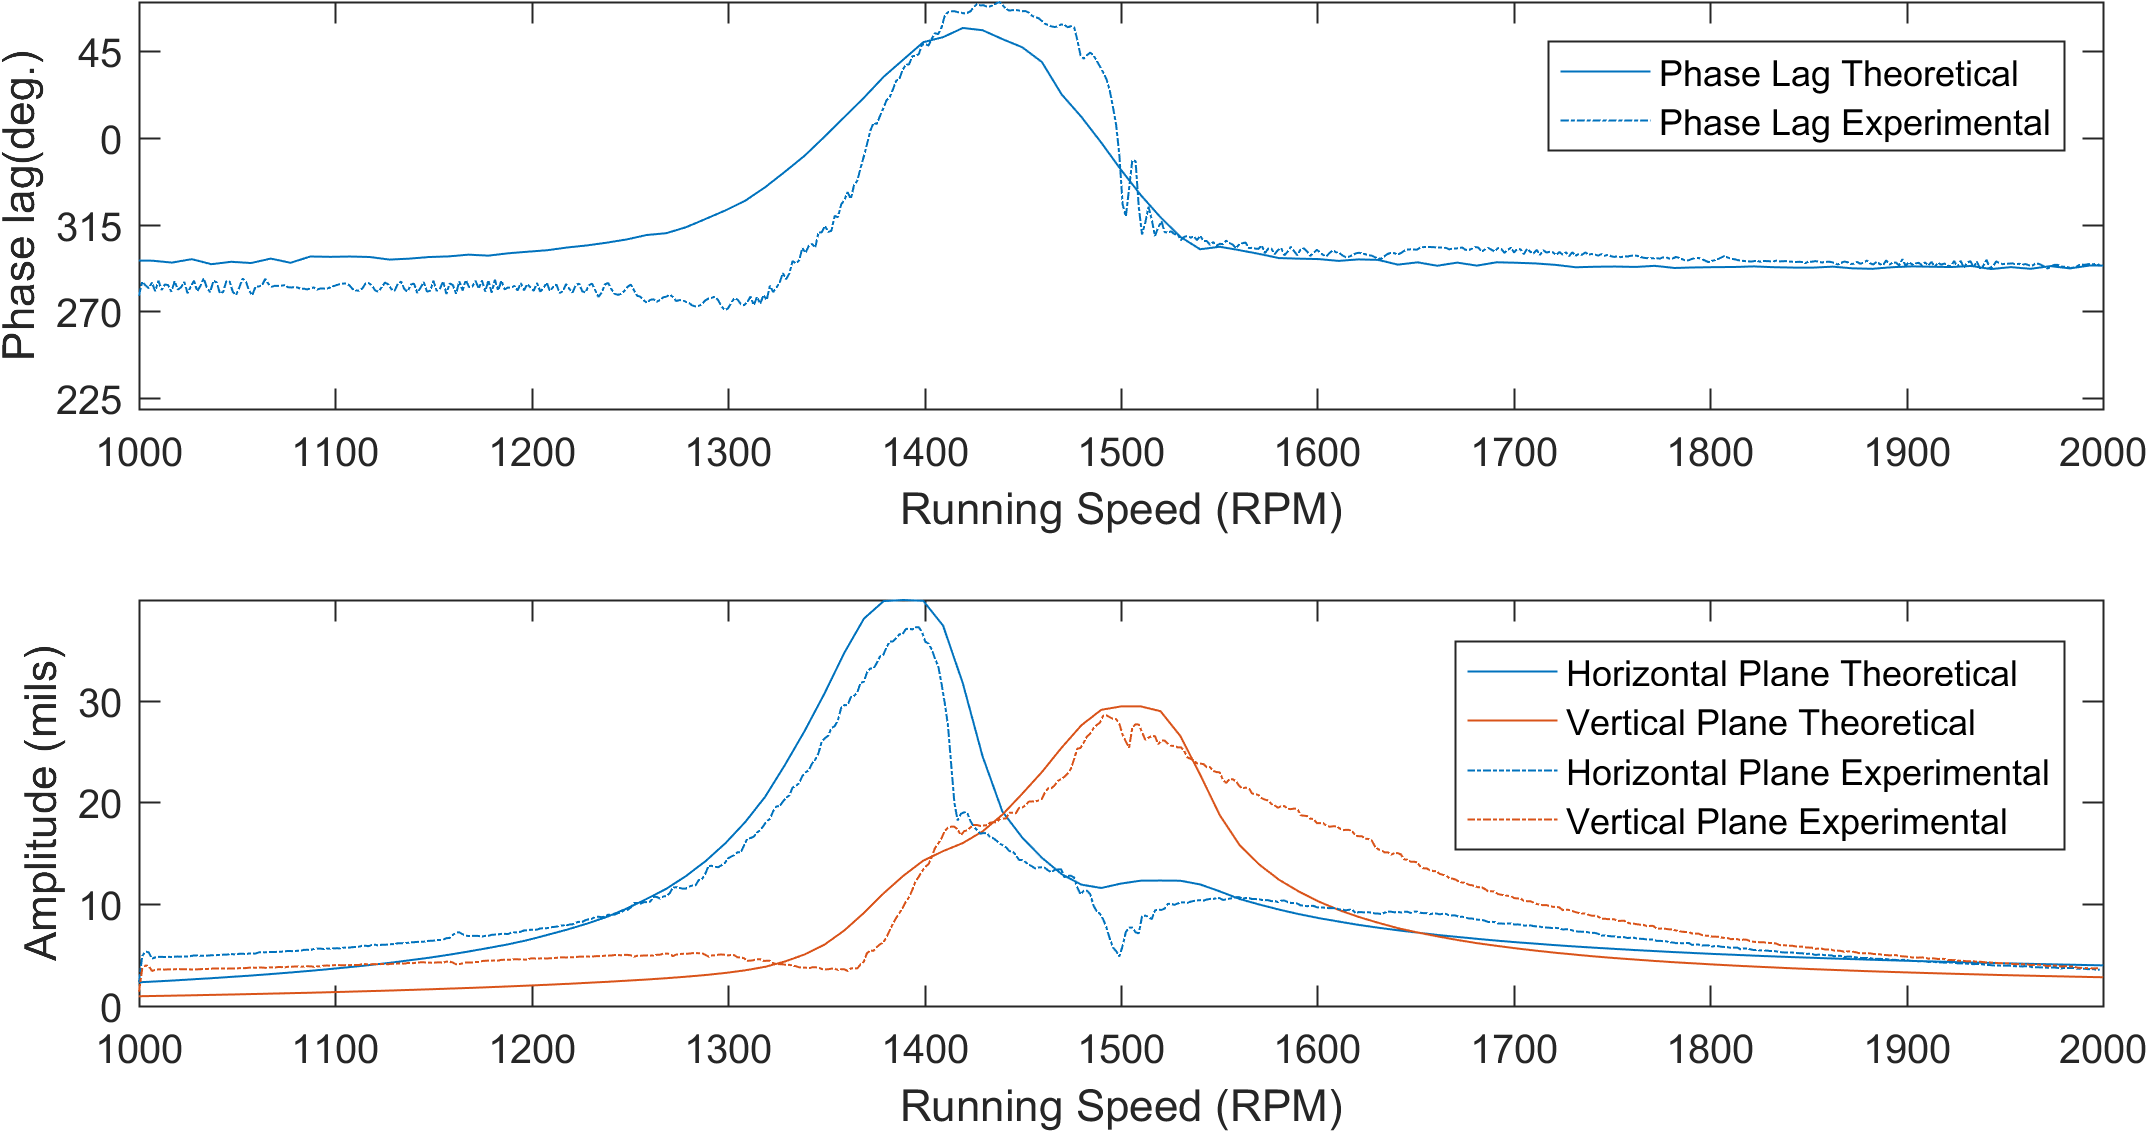
\includegraphics[width=1\linewidth]{./figures/Images/Figure_14}
			\caption{Bode plot, Experimental vs. Theoretical}
			\label{fig:Figure_14}
		\end{figure}
		The Bode plot of Figure \ref{fig:Figure_14} compares the startup amplitude and phase angle of the theoretical model and the experiment. Because both the experimental and the theoretical results were processed using our strategy with the same MATLAB code to produce these plots, comparisons can be confidently drawn. The phase angles are of a phase lag from the X transducer and from the Y transducer. The two transducers are 270 positive degrees apart around the shaft.\par 
		\begin{figure}[H]	
			\centering
			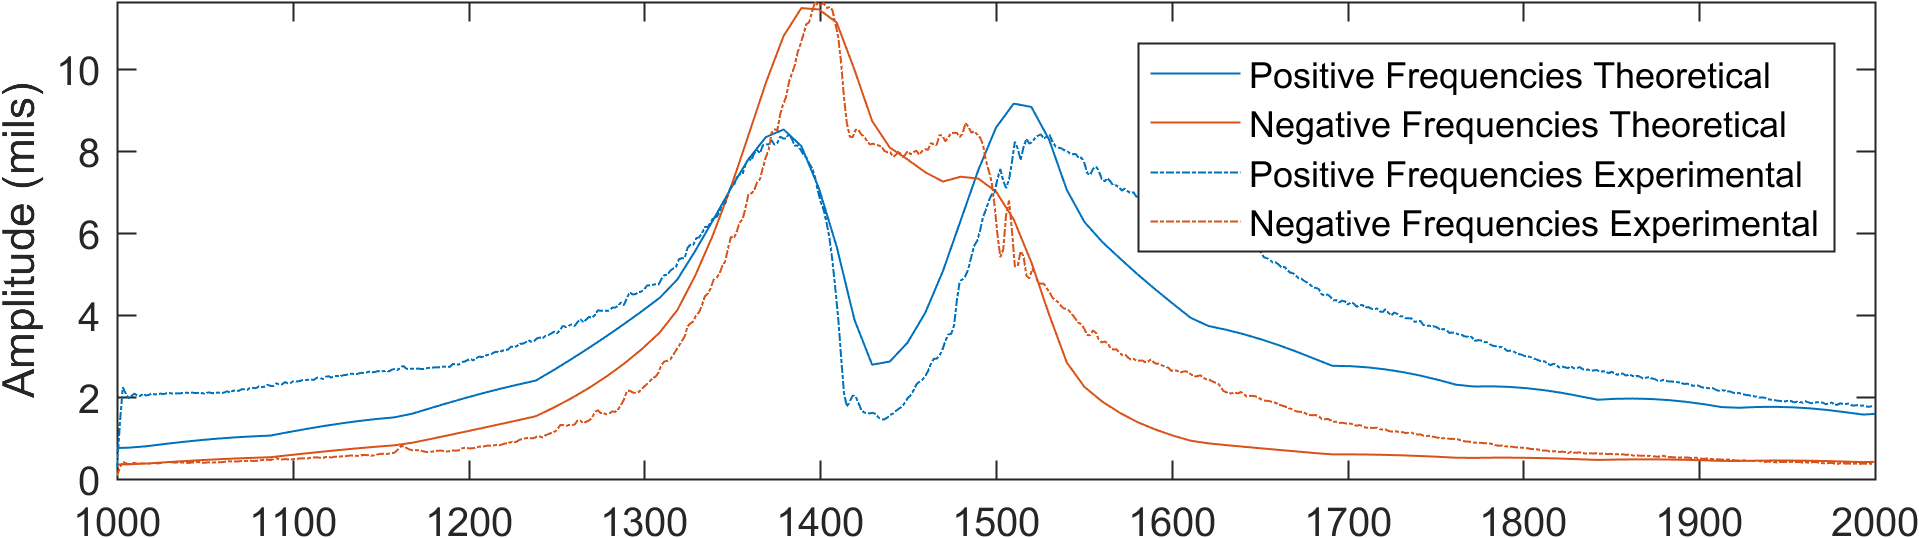
\includegraphics[width=1\linewidth]{./figures/Images/Figure_15}
			\caption{Positive/Negative frequency comparison, Experimental vs. Theoretical}
			\label{fig:Figure_15}
		\end{figure}
		Observing the comparison of positive and negative frequencies as done in Figure \ref{fig:Figure_15} allows the detection of backward or forward whirl. When the negative frequency amplitude is greater than that of the positive frequency, the whirl is “backward”. Backward whirl describes the phenomenon of precession of the shaft vibration rotating opposite to the rotation of the shaft. Comparison to the typical horizontal vs. vertical amplitude plot shows that the crossover from positive to negative whirl occurs when either the horizontal or vertical vibration amplitudes drop.\par 
		\begin{figure}[H]
			\begin{subfigure}[b]{.5\linewidth}	
				\centering
				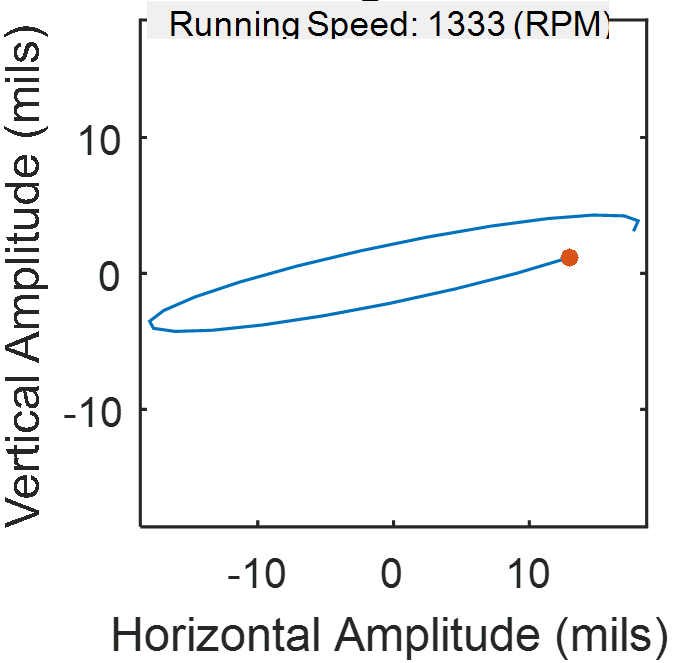
\includegraphics[width=.75\textwidth]{./figures/Images/Figure_16a}
				\caption{Experimental 1333 RPM orbit}
				\label{fig:Figure_16a}
			\end{subfigure}
			\begin{subfigure}[b]{.5\linewidth}
				\centering
				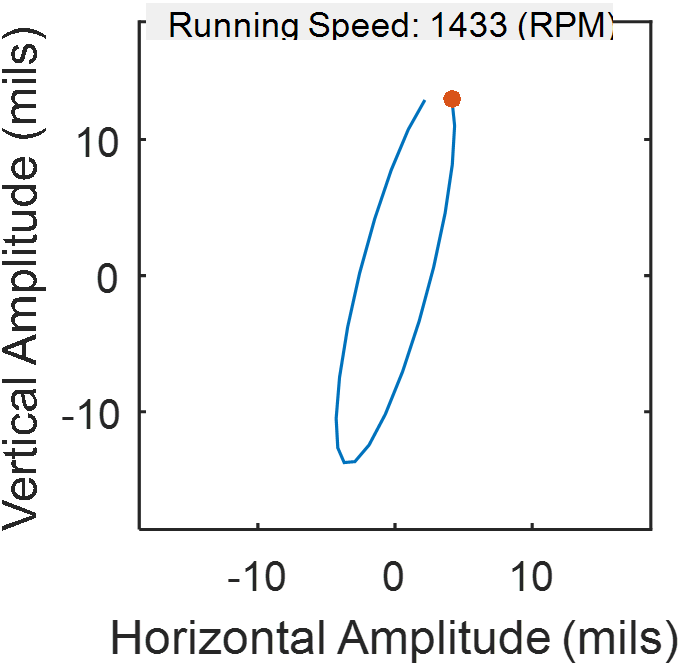
\includegraphics[width=.75\textwidth]{./figures/Images/Figure_16b}
				\caption{Experimental 1433 RPM orbit}
				\label{fig:Figure_16b}
			\end{subfigure}
			\begin{subfigure}[b]{.5\linewidth}
				\centering
				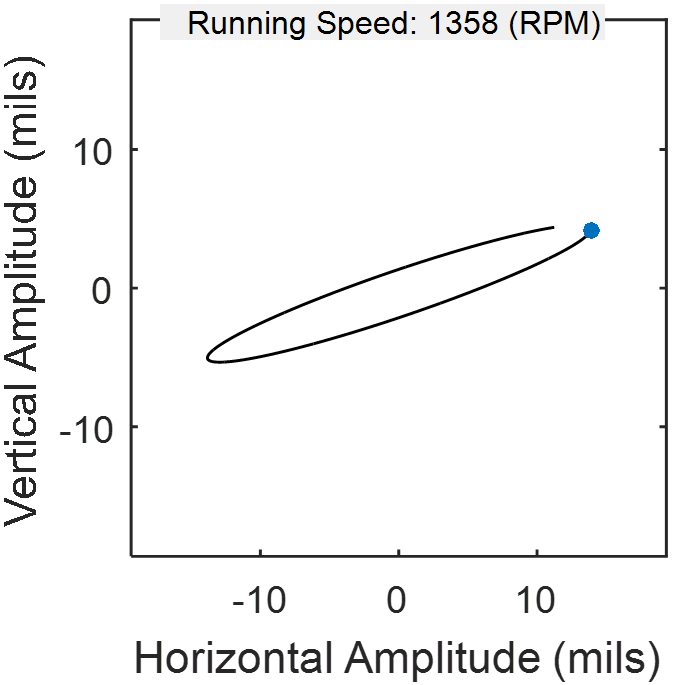
\includegraphics[width=.75\textwidth]{./figures/Images/Figure_16c}
				\caption{Theoretical 1358 RPM orbit}
				\label{fig:Figure_16c}
			\end{subfigure}
			\begin{subfigure}[b]{.5\linewidth}
				\centering
				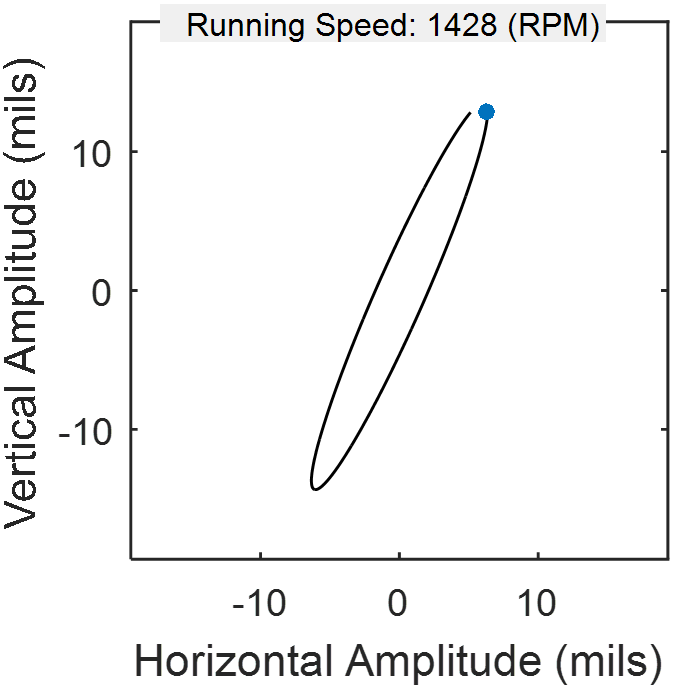
\includegraphics[width=.75\textwidth]{./figures/Images/Figure_16d}
				\caption{Theoretical 1428 RPM orbit}
				\label{fig:Figure_16d}
			\end{subfigure}
			\caption{Orbit plots fo filtered experimental data compared to theoretical predictions at similar speeds}
			\label{fig:Figure_16}
		\end{figure}
		Orbit plots of Figure \ref{fig:Figure_16} are created using experimental and theoretical data. The orbits of experimental data contain the key-phasor dot to mark the beginning of a rotation from a fixed location on the shaft. This allows the determination of the orbit rotation direction. For all of the orbit plots, the shaft was rotating in the counter-clockwise direction. Therefore, an orbit in the clockwise direction is in the “reverse” direction. Experimental data was filtered using a tracking filter for the orbit plots. Since a once per turn reference is unavailable for theoretical data, the orbits are plotted with a reference dot at the maximum $x$ value for that orbit.\par 
		\begin{figure}[H]	
			\centering
			\includegraphics[width=1\linewidth]{./figures/Images/Figure_17}
			\caption{Experimental 3D Orbit plot produced by our strategy}
			\label{fig:Figure_17}
		\end{figure}
		\begin{figure}[H]	
			\centering
			\includegraphics[width=1\linewidth]{./figures/Images/Figure_18}
			\caption{Theoretical 3D Orbit plot}
			\label{fig:Figure_18}
		\end{figure}
		Orbit plots are cascaded in increasing rotational speed in the 3D orbit plots of Figures \ref{fig:Figure_17} and \ref{fig:Figure_18}. This cascade of orbits gives a sense of how the natural frequencies are physically manifested in these startups. This 3D orbit plot lends a more intuitive representation of the data and at the same time, important characteristics such as phase lag, amplitudes and reverse precession can be discerned from the plot. This plot was also useful in comparing the theoretical model to the experimental data, because it demonstrates magnitude as well as general shape of the response of the entire orbit in one plot. Also Figure \ref{fig:Figure_17} and \ref{fig:Figure_18} makes clear the effect of gyroscopic moments, as the shape of the elliptical orbits during peak amplitude vibrations are bent. The ADRE Sxp software does not produce this plot.\par 
	\section{Discussion and conclusions}
		3D cascade plots (Figures \ref{fig:Figure_12}, \ref{fig:Figure_13}) produced using our complex FFT strategy clearly display the full vibration spectrum and complement those produced with the ADRE Sxp software (Figure \ref{fig:Figure_11}). Both the theoretical model and the experimental results display a sudden dip in amplitude of positive frequencies between the two natural frequencies (Figures \ref{fig:Figure_12},\ref{fig:Figure_13}). This dip is coupled with an increase in negative frequencies, resulting in reverse orbits for a period in time. These negative orbits can be seen in Figure \ref{fig:Figure_16}. The theoretical model suggested a strong influence from the relative phase angle of the skew to the eccentricity. Some values of phase difference offered completely positive orbits through the natural frequency, while others offered highly negative orbits. This is the greatest contribution from the skew angle, as without the consideration of it, the amount of negative to positive vibration could not be easily altered in the theoretical model.\par 
		In this paper, the dynamic behavior of a flexible shaft with an overhung disk has been studied by employing full spectrum analysis. Anisotropic bearing stiffness and the effect of gyroscopic moments are considered in our classic theoretical model. Some of the parameters which are difficult to directly measure are estimated by combination of theoretical calculation and experimental results. Full spectrum analysis is applied to the system to reveal some interesting backward whirl vibration phenomena due to the interaction of anisotropy of the stiffness of the bearings, flexibility of the shaft and gyroscopic effect. Phenomena such as these cannot be disclosed by traditional half spectrum FFT. 3D cascade full spectrum plots from theoretical model are compared to those from experiments. Our full spectrum cascade plots using complex FFT strategy capture more detail in the vibration response of the system than the typical cascade plots. Filtered orbit plots with the key-phasor dots at different speed demonstrate forward and backward whirls. Methods for identifying the eccentricity and skew angle of the disk are presented. Also, the effect of the skew angle is determined by comparison of experiment and theory. The skew angle is determined by comparing theoretical angular amplitudes to experimental angular amplitudes. Bearing stiffness is determined through a method of matching theoretical and experimental natural frequencies. Consideration of the gyroscopic moments introduces speed as another dependent variable in the equation for natural frequency, making the process of matching an iterative one.\par 
	\section{Acknowledgments}
		The authors acknowledge the Donald E. Bently Center for Engineering Innovation at California Polytechnic State University San Luis Obispo for support of this work.\par 